% PAQUETES
\documentclass[a4paper, 10pt, onecolumn,journal]{ieeeconf}
\overrideIEEEmargins
\usepackage[utf8]{inputenc}
\usepackage[T1]{fontenc}
\usepackage{fancyhdr}
\usepackage{lastpage}
\usepackage{graphicx}
\usepackage{amsmath}
\usepackage{amssymb} % Para símbolos matemáticos adicionales
\usepackage{adjustbox}
\usepackage{cleveref}
\usepackage{array}
\newcommand{\defeq}{\mathrel{\mathop:}=}
\newcolumntype{C}[1]{>{\centering\arraybackslash}m{#1}}
\renewcommand{\arraystretch}{1.5} % Ajusta este valor para más o menos espacio entre filas
\usepackage[prepend]{epstopdf}
\graphicspath{{imágenes/}} 


% Configuración del encabezado y el pie de página
\pagestyle{fancy}
\fancyhf{}

% Encabezado
\fancyhead[L]{UNCuyo -- Ing. Mecatrónica \\ Mendoza - Argentina}
\fancyhead[C]{\textbf{311 -- AUTOMÁTICA Y MÁQUINAS ELÉCTRICAS \\ PROYECTO GLOBAL INTEGRADOR}}
\fancyhead[R]{Año: 2024 \\ Alumnos: Borquez y Escobar\\Fecha: 06/06/2024}

% Pie de página
\fancyfoot[C]{Página \thepage\ de \pageref{LastPage}} % Muestra "Página x de xx"

% Línea en la parte superior del encabezado
\renewcommand{\headrulewidth}{0.4pt}

% Línea en la parte inferior del pie de página
\renewcommand{\footrulewidth}{0.4pt}

% TÍTULO
\title{\LARGE \bf
Proyecto Global Integrador: Control de Accionamiento de CA con
Motor Sincrónico de Imanes Permanentes
}

% AUTORES
\author{Borquez Juan y Escobar Matías}

% INICIO DEL DOCUMENTO
\begin{document}

\maketitle
\thispagestyle{empty}
\pagestyle{fancy}

% RESUMEN
\begin{abstract}
\end{abstract}

% INTRODUCCIÓN
\section{INTRODUCCIÓN}
Modelado, simulación, diseño y análisis de desempeño de un Sistema de Control Automático de Posición y Movimiento para un Accionamiento electromecánico de 4 cuadrantes, compuesto por: máquina eléctrica de corriente alterna (CA) trifásica sincrónica con excitación por imanes permanentes (PMSM), alimentada por inversor trifásico desde fuente de corriente continua (CC); reductor de velocidad de engranajes planetarios de salida hacia la carga mecánica; realimentación con 1 sensor de posición en el eje del motor, más 3 sensores de corriente instantánea de fases en la salida del inversor trifásico al estator de la máquina (PMSM) y 1 sensor de temperatura del bobinado de estator.

% ECUACIONES
\section{ECUACIONES}
Se detallan en esta sección las ecuaciones que modelan las distintas partes del sistema, obtenidas de la guía de referencia (\cite{c1}) en donde también se detalla claramente el significado de cada uno de los términos en las ecuaciones.


\begin{itemize}
    % carga
    \item Modelo matemático simplificado equivalente no lineal de parámetros variables referido al eje de salida del tren de transmisión:
    \begin{equation}
        J_l \frac{d\omega_l(t)}{dt} = T_q(t) - b_l \omega_l(t) - T_l(t)
        \label{carga mecanica}
    \end{equation}
    \begin{equation}
        T_l(t) = k_l \sin(\theta_l(t)) + T_d(t)
        \label{torque de carga}
    \end{equation}
    \begin{equation}
        \frac{d\theta_l(t)}{dt} \equiv \omega_l(t) \Leftrightarrow \theta_l(t) = \int_{0}^{t} \omega_l(\zeta) \, d\zeta + \theta_l(0)
        \label{velocidad y posición de la carga}
    \end{equation}

    % transmisión
    \item Modelo equivalente rígido del tren de transmisión:
    \begin{equation}
        \omega_l(t) = 1/r \cdot \omega_m(t)
        \label{relacion de velocidad en caja}
    \end{equation}
    \begin{equation}
        T_q(t) = r \cdot T_{dm}(t)
        \label{relacion de torque en caja}
    \end{equation}
    
    % sub-sistema mecánico PMSM
    \item Modelo matemático equivalente del sub-sistema mecánico de la máquina eléctrica.
    \begin{equation}
        J_m \frac{d\omega_m(t)}{dt} = T_m(t) - b_m \omega_m(t) - T_{dm}(t)
        \label{subsistema mecanico maquina electrica}
    \end{equation}
    \begin{equation}
        \frac{d\theta_m(t)}{dt} \equiv \omega_m(t) \Leftrightarrow \theta_m(t) = \int_{0}^{t} \omega_m(\tau) d\tau + \theta_m(0)
        \label{posicion y velocidad motor}
    \end{equation}

    % sub-sistema electromagnético PMSM
    \item Coordenadas eléctricas de entrehierro $qd0^{r}$ (marco de referencia de rotor $\neq$ “sincrónico”):
    \begin{equation}
        \frac{d\theta_r(t)}{dt} \equiv \omega_r(t) \Leftrightarrow \theta_r(t) = \int_{0}^{t} \omega_r(\tau) d\tau + \theta_r(0)
        \label{Relacion coordenadas electricas y mecanicas}
    \end{equation}
    \begin{equation}
        \theta_r(t) \equiv P_p \theta_m(t) \therefore  \omega_r(t) = P_p \omega_m(t)
        \label{posicion y velocidad rotor}
    \end{equation}
    \item Torque electromagnético:
    \begin{equation}
        T_m(t) = \frac{3}{2} P_p [\lambda'^r_{m} i^r_{qs}(t) + (L_d - L_q) i^r_{ds}(t) i^r_{qs}(t)]
        \label{torque electromagnetico}
    \end{equation}
    \item Balance de tensiones eléctricas equivalentes de estator (referido a coordenadas $qd0^{r}$):
    \begin{equation}
        v^r_{qs}(t) = R_s(t) i^r_{qs}(t) + L_q \frac{di^r_{qs}(t)}{dt} + [\lambda'^r_{m} + L_d i^r_{ds}(t)] \omega_r(t)
        \label{balance de tensiones q}
    \end{equation}
    \begin{equation}
        v^r_{ds}(t) = R_s(t) i^r_{ds}(t) + L_d \frac{di^r_{ds}(t)}{dt} - L_q i^r_{qs}(t) \omega_r(t)
        \label{balance de tensiones d}
    \end{equation}
    \begin{equation}
        v_{0s}(t) = R_s(t) i_{0s}(t) + L_{ls} \frac{di_{0s}(t)}{dt}
        \label{balance de tensiones 0}
    \end{equation}

    % Sub-sistema térmico
    \item Modelo matemático de variación de la resistencia eléctrica del bobinado con la temperatura.
    \begin{equation}
        R_s(t) = R_{sREF} \left(1 + \alpha_{Cu} (T_s^{\circ}(t) - T_{sREF}^{\circ})\right)
        \label{Rs}
    \end{equation}

    \item Potencia de pérdidas calóricas:
    \begin{equation}
        P_{s\ perd}(t) = R_s(t) \left(i_{as}^2(t) + i_{bs}^2(t) + i_{cs}^2(t)\right) = \frac{3}{2} R_s(t) \left(i_{qs}^2(t) + i_{ds}^2(t) + 2 i_{0s}^2(t)\right)
        \label{potencia de perdidas}
    \end{equation}
    \item Balance térmico de estator:
    \begin{equation}
        P_{s\ perd}(t) = C_{ts} \frac{dT_s^{\circ}(t)}{dt} + \frac{1}{R_{ts-amb}} \left(T_s^{\circ}(t) - T_{amb}^{\circ}(t)\right)
        \label{balance termico estator}
    \end{equation}

    % Variables del modelo
    \item Vector de estado del sistema físico completo.
    \begin{equation}
        \mathbf{x}(t) = \begin{bmatrix} \theta_m(t) \\ \omega_m(t) \\ i^r_{qs}(t) \\ i^r_{ds}(t) \\ i_{0s}(t) \\ T_s(t) \end{bmatrix}
        \label{vector de estado del sistema}
    \end{equation}
    \item Vector de entradas de manipulación al modelo dinámico del sistema físico completo en coordenadas virtuales y reales respectivamente
    \begin{equation}
        \mathbf{u_{c(qd0)}}(t) = \begin{bmatrix} v^r_{qs}(t) \\ v^r_{ds}(t) \\ v^r_{0s}(t)\end{bmatrix}
        \mathbf{u_{c(abc)}}(t) = \begin{bmatrix} v_{as}(t) \\ v_{bs}(t) \\ v_{cs}(t)\end{bmatrix}
        \label{vector de entradas de control}
    \end{equation}
    \item Vector de entradas de perturbación al modelo dinámico del sistema físico completo.
    \begin{equation}
        \mathbf{u_{d}}(t) = \begin{bmatrix} T_l(t) \\ T_{amb}^{\circ}(t)\end{bmatrix}
        \label{vector de entradas de perturbacion}
    \end{equation}
    \item Vector de entradas total al modelo dinámico del sistema físico completo.
    \begin{equation}
        \mathbf{u}(t) = \begin{bmatrix} \mathbf{u_c}(t) \\ \mathbf{u_d}(t)\end{bmatrix} \, \, \, \,
        \mathbf{u}(t) = \begin{bmatrix} v^r_{qs}(t) \\ v^r_{ds}(t) \\ v^r_{0s}(t) \\ T_l(t) \\ T_{amb}^{\circ}(t) \end{bmatrix}\, \, \, \,
        \mathbf{u}(t) = \begin{bmatrix} v_{as}(t) \\ v_{bs}(t) \\ v_{cs}(t)\\ T_l(t) \\ T_{amb}^{\circ}(t) \end{bmatrix}
        \label{vector de entradas}
    \end{equation}
    % Inversor trifásico.
    \item Sistema de tensiones trifásico a la salida del inversor.
    \begin{align}
        v_{as}(t) &\approx \frac{\sqrt{2}}{\sqrt{2}} \cdot V_{sl}(t) \cdot \cos(\theta_{ev}(t)) \quad \text{(Ec. 4.1)} \\
        v_{bs}(t) &\approx \frac{\sqrt{2}}{\sqrt{2}} \cdot V_{sl}(t) \cdot \cos\left(\theta_{ev}(t) - \frac{2\pi}{3}\right) \quad \text{(Ec. 4.2)} \\
        v_{cs}(t) &\approx \frac{\sqrt{2}}{\sqrt{2}} \cdot V_{sl}(t)\cdot \cos\left(\theta_{ev}(t) + \frac{2\pi}{3}\right) \quad \text{(Ec. 4.3)} \\
        \label{sistema de tensiones trifásico real}
    \end{align}
    \item Frecuencia eléctrica del sistema de tensiones trifásico y ángulo eléctrica
    \begin{align}
        \omega_e(t) &\equiv 2\pi \cdot f_e(t) \equiv \frac{d\theta_{ev}(t)}{dt} \iff \theta_{ev}(t) = \int_{0}^{t} \omega_e(\xi) \, d\xi + \theta_{ev}(0)
        \label{frecuencia eléctrica y ángulo eléctrico}
    \end{align}
    \item Ángulo de carga de la máquina eléctrica:
    \begin{equation}
        \delta(t) \equiv \theta_r(t) - \theta_{ev}(t) = \int_{0}^{t} [\omega_r(\xi) - \omega_e(\xi)] \, d\xi + \theta_r(0) - \theta_{ev}(0)
        \label{ángulo de carga}
    \end{equation}
\end{itemize}

% DESARROLLO - PRESENTACIÓN DEL PROBLEMA
\section{PRESENTACIÓN DEL PROBLEMA}
El problema bajo estudio se encuentra bien detallado en la guía de referencia (\cite{c1}), por lo que en esta sección se indican solo los aspectos más relevantes de cada una de las partes del problema, sin hacer énfasis en las ecuaciones que describen los modelos de cada una de las partes ni en los parámetros de cada uno de los subsistemas.

% Carga mecánica
\subsection{\textbf{carga mecánica}}
Aplicación simplificada de referencia (adaptado de \cite{c2}): control de movimiento de 1 eje (descentralizado) para articulación de brazo manipulador robótico elemental de un grado de libertad (1 g.d.l.) rotacional de eje horizontal sometido a la acción de la aceleración de gravedad (péndulo rígido actuado), con eje de rotación fijo a base en sistema de referencia inercial (\cref{brazo}); con parámetros equivalentes variables según sea la carga útil transportada en el extremo.

\begin{figure}[thpb]
    \centering
    \begin{adjustbox}{max width=0.5\columnwidth}
        \framebox{\parbox{\columnwidth}{
            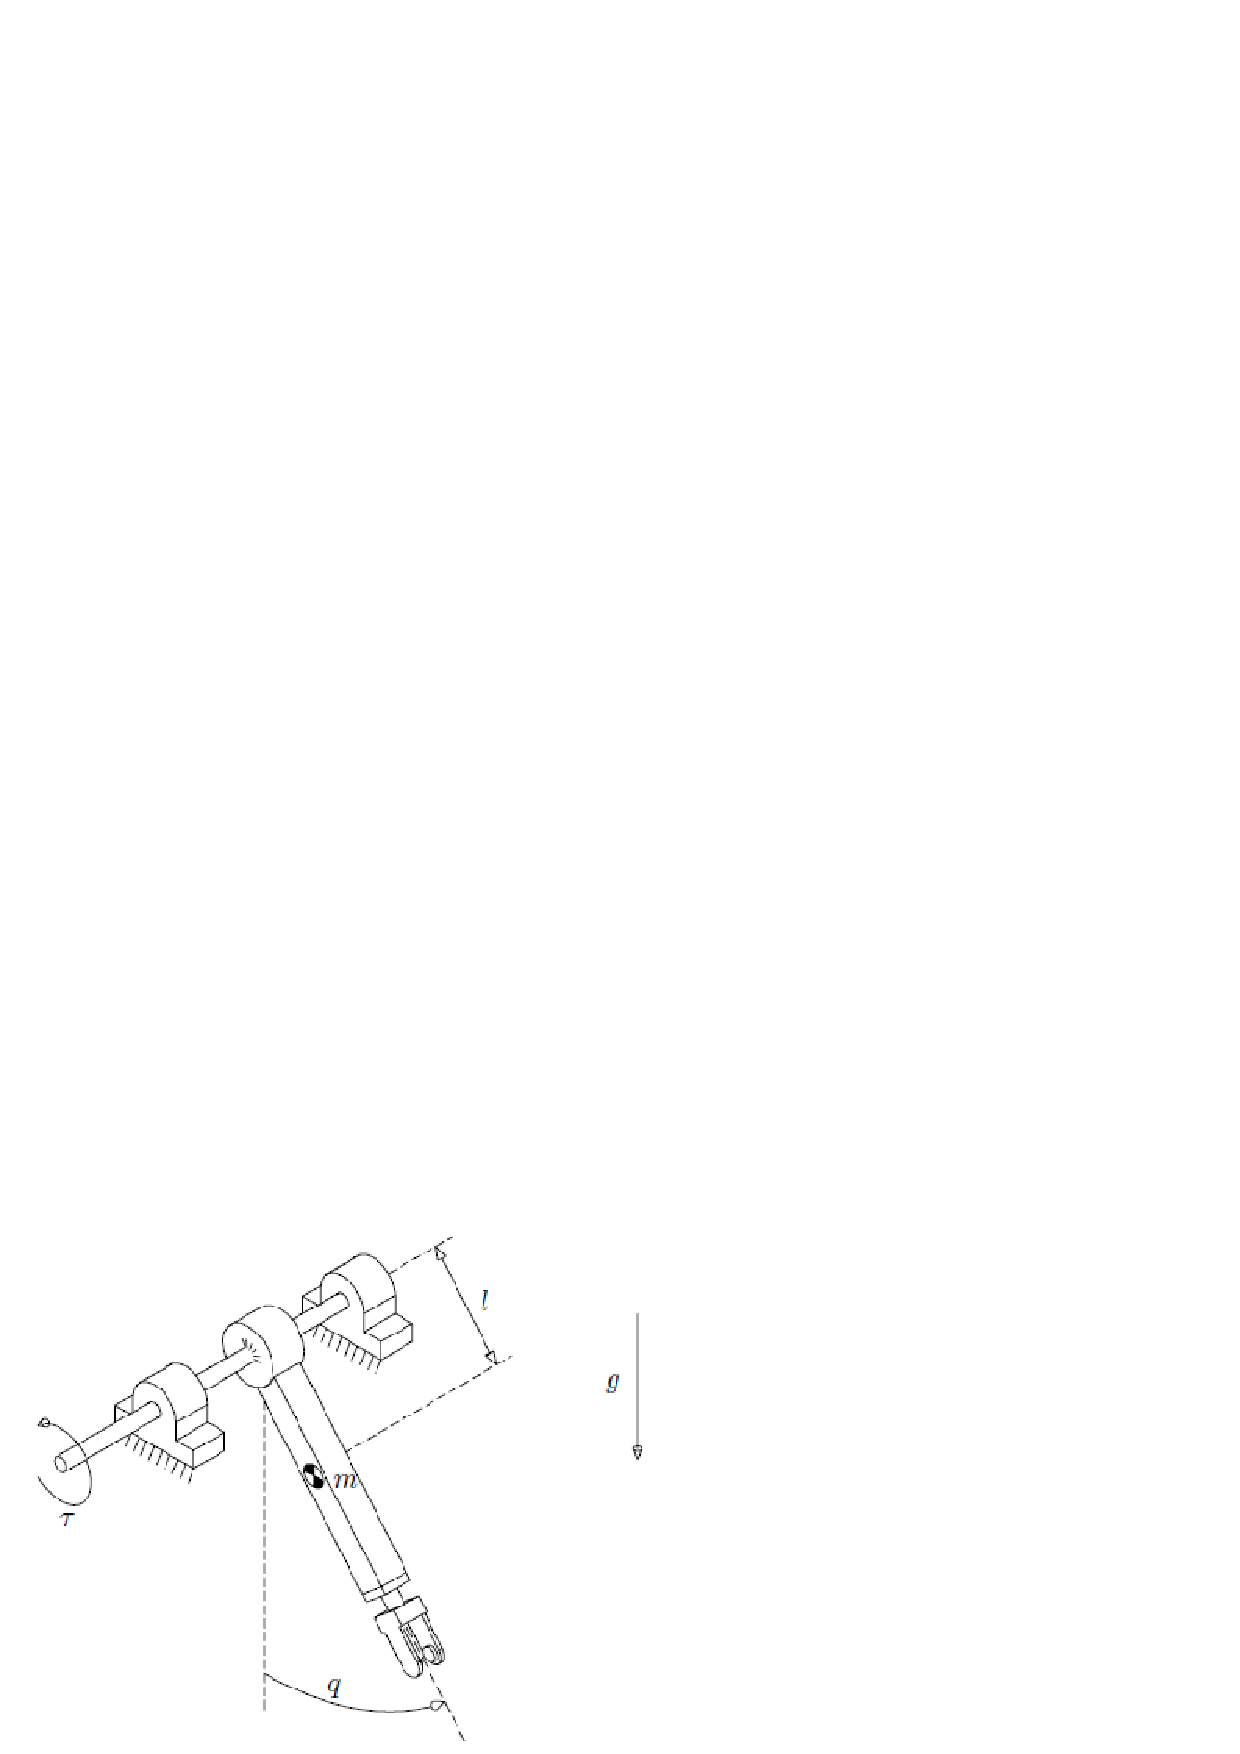
\includegraphics[width=\columnwidth]{1-Brazo.PNG}
        }}
    \end{adjustbox}
    \caption{Robot manipulador elemental de 1 g.d.l. en plano vertical (péndulo rígido actuado) \cite{c2}.}
    \label{brazo}
\end{figure}

% Caja reductora
\subsection{\textbf{Caja Reductora}}
Caja reductora reversible con sistema de engranajes planetarios, asumiendo acoplamiento rígido (sin elasticidad torsional y sin juego, holgura o ``backlash''); momento de inercia equivalente y pérdidas de energía por fricción interna, reflejados al eje de entrada y considerados junto con el motor

% Máquina eléctrica PMSM
\subsection{\textbf{Máquina Eléctrica PMSM}}
Máquina eléctrica de CA trifásica sincrónica con excitación por imanes permanentes (PMSM) y estator conectado en estrella (simétrico y equilibrado) accesible en bornes de fases $abc$, con centro de estrella (punto “neutro”) flotante (no accesible).

% Subsistema térmico de la máquina eléctrica
\vspace*{0.2cm}
\subsubsection{\textbf{subsistema térmico}} Modelo simplificado equivalente de primer orden, considerando sólo pérdidas
eléctricas resistivas por efecto Joule en bobinado de estator, despreciando pérdidas magnéticas
en el núcleo; transferencia de calor por conducción y convección natural, sin ventilación forzada.

% Inversor trifásico
\subsection{\textbf{Inversor trifásico de alimentación (modulador de tensión)}}

Inversor trifásico de 4 cuadrantes (regenerativo), consistente en puente trifásico con llaves electrónicas semiconductoras alimentado desde fuente de CC de tensión constante, conmutado con modulación de ancho de pulso.

No es parte de este proyecto el análisis del detalle de operación del inversor ni su fuente de energía de CC. Se considera al inversor trifásico y la fuente de CC como un Modulador idealizado de tensión trifásico (vectorial) (modelo promediado que se indica a continuación) para alimentación al estator de la Máq. Eléctrica.


\subsubsection{\textbf{Modelo Promediado}}
Se considera un modelo promediado equivalente de tensiones sintetizadas de salida (componente fundamental, sin armónicos). Se trata de un sistema trifásico de tensiones de fase en bornes de estator, senoidales de secuencia positiva $abc$, equilibrado o balanceado, variable en Módulo $V_{sl}(t)$ y Frecuencia $\omega_e(t)$.

% SENSORES
\subsection{\textbf{Sensores de retroalimentación}}

El sistema cuenta con los siguientes dispositivos físicos y sus canales de medición y acondicionamiento:
\begin{itemize}
    \item 1 sensor de posición angular (codificador incremental o “encoder”) montado en el eje de motor, asumiendo proceso de “homming” y decodificación idealizados. Se logra la medición de la posición angular absoluta “rectificada” (al girar más de una revolución)
    \[\rightarrow \text{variable medida}: \theta_m(t)\]
    \item 3 sensores de corriente instantánea de fase, montados en salida trifásica del inversor hacia bornes del estator.
    \[\rightarrow \text{variables medidas}: i_{as}(t), i_{bs}(t), i_{cs}(t)\]
    \item 1 sensor de temperatura (ej. RTD) en bobinado de estator. Se mide la temperatura para monitoreo de calentamiento y estimación de resistencia de estator $R_s(t)$.
    \[\rightarrow \text{variable medida}: T_s^{\circ}(t)\]
\end{itemize}

% VARIABLES DE ESTADO UTILIZADAS EN EL MODELO
\subsection{\textbf{Variables principales en el Modelo Dinámico completo}}
Se utilizan las siguientes variables para representar el estado, las entradas y las salidas en el modelo del sistema dinámico completo.

\textbf{a) Excitaciones (entradas) externas:}
\begin{itemize}
    \item Variable manipulada (vectorial): Sistema trifásico de tensiones de fase reales en bornes de estator $v_{abc}(t)$, con $V_{sl}(t)$ y $\omega_e(t)$ ajustables a través de manipulación de la modulación PWM del inversor.
    \item Variables de perturbación: Torque externo de carga mecánica $T_l(t)$ aplicado en la articulación del brazo manipulador. Temperatura ambiente $T_{amb}^{\circ}(t)$.
\end{itemize}

\textbf{b) Estado interno:}
\begin{itemize}
    \item Posición $\theta_m(t)$ y velocidad $\omega_m(t)$ en eje del motor. Corrientes virtuales equivalentes de estator $i_{qd0s}^r(t)$; temperatura de estator $T_s^{\circ}(t)$.
\end{itemize}

\textbf{c) Respuestas (salidas) externas:}
\begin{itemize}
    \item Variable controlada, no medida directamente (efector final): Posición angular de eje de la carga $q(t) \equiv \theta_l(t)$.
    \item Variables medidas (para realimentación): Posición angular de eje del motor $\theta_m(t)$. Sistema trifásico de corrientes de fase reales en bornes de estator $i_{abc}(t)$. Temperatura de estator $T_s^{\circ}(t)$.
\end{itemize}

% DESARROLLO DE LAS TAREAS
\section{DESARROLLO DE TAREAS}

%5.1
\subsection{\textbf{Modelado, Análisis y Simulación dinámica del SISTEMA FÍSICO a “Lazo Abierto” (Sin Controlador externo de Movimiento)}}

%5.1.1
\subsubsection{\textbf{Modelo sub-sistema mecánico completo referido al eje de la máquina eléctrica}}

Multiplicando por $r$ ambos miembros de la \cref{subsistema mecanico maquina electrica}, sumando miembro a miembro con la \cref{carga mecanica} y tomando en cuenta $T_q(t)$ según \cref{relacion de torque en caja} obtenemos:

\begin{flalign*}
    J_{l}\,\frac{d\omega _{l}\left(t\right)}{dt} +J_{m}\,r\,\frac{d\omega _{m}\left(t\right)}{dt} =r\,T_{m}\left(t\right)-T_{l}\left(t\right)-b_{l}\,\omega _{l}\left(t\right)-b_{m}\,r\,\omega _{m}\left(t\right)
\end{flalign*}

Reemplazando en la anterior $\omega_{l}(t)$ según \cref{relacion de velocidad en caja}, agrupando términos y diviendo entre $r$ a ambos miembros, obtenemos:

\begin{flalign}
    \left(J_{m}+\frac{J_{l}}{r^2}\right)\,\frac{d \omega _{m}\left(t\right)}{dt}=T_{m}\left(t\right)-\left(b_{m}+\frac{b_{l}}{r^2}\right)\,\omega _{m}\left(t\right)-\frac{T_{l}\left(t\right)}{r}
    \label{subsistema mecanico con parametros desarrollados}
\end{flalign}

Definimos ahora la inercia equivalente y el amortiguamiento equivalente respectivamente como:

\begin{equation}
   J_{eq}= \left(J_{m}+\frac{J_{l}}{r^2}\right)
   \label{inercia equivalente}
\end{equation}

\begin{equation}
    b_{eq}=\left(b_{m}+\frac{b_{l}}{r^2}\right)
    \label{amortiguamiento equivalente}
\end{equation}

Reemplazando la \cref{inercia equivalente} y la \cref{amortiguamiento equivalente} en la \cref{subsistema mecanico con parametros desarrollados} obtenemos el modelo matemático equivalente del sub-sistema mecánico completo con parámetros equivalentes referido al eje del motor (véase diagrama de bloques de la \cref{diagrama de bloques sub-sistema mecanico completo}):
\begin{flalign}
    J_{eq}\,\frac{d \omega _{m}\left(t\right)}{dt}=T_{m}\left(t\right)-b_{eq}\, \omega _{m}\left(t\right)-\frac{T_{l}\left(t\right)}{r}
    \label{subsistema mecanico con parametros equivalentes}
\end{flalign}

\begin{figure}[thpb]
    \centering
    \begin{adjustbox}{max width=\columnwidth}
        \framebox{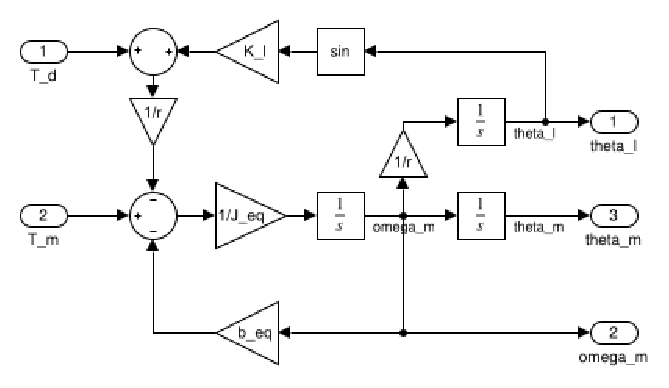
\includegraphics{2-Subsistema_Mecánico_Completo.eps}}
    \end{adjustbox}
    \caption{Diagrama de bloques del sub-sistema mecánico completo.}
    \label{diagrama de bloques sub-sistema mecanico completo}
\end{figure}

El modelo resultante tiene un solo grado de libertad, tal como sucede en el modelo de la
carga y en el del subsistema mecánico de la máquina eléctrica sin la transmisión.
Esto se debe a la suposición de rigidez ideal y la ausencia de "backlash" en la reducción, 
permitiendo un "acoplamiento directo" de la carga al eje de la máquina.
Dicho de otra manera, la transmisión no incorpora dinámica al subsistema mecánico.

%5.1.2

\subsubsection{\textbf{Modelo dinámico del sistema físico completo}} este incorpora los sub-sistemas electromagnético, mecánico y térmico.

% a
\paragraph{\textbf{Modelo Global No Lineal}}
Al tratarse de un sistema no lineal de parámetros variables y con no-linealidades en las variables de estado, no se puede obtener una expresión
de la ecuación de estado y de salida del sistema en la forma:

\begin{equation*}
    \begin{cases}
        \frac{d \mathbf{x}(t)}{dt} = A \mathbf{x}(t) + B \mathbf{u}(t)\\
        \mathbf{y}(t) = C \mathbf{x}(t) + D \mathbf{u}(t)
    \end{cases}
\end{equation*}

Sin embargo, se puede obtener una expresión del modelo matemático vectorial en la forma más general:

\begin{equation*}
    \begin{cases}
        \frac{d \mathbf{x}(t)}{dt} = f(\mathbf{x}(t), \mathbf{u}(t), t)\\
        \mathbf{y}(t) = g(\mathbf{x}(t), \mathbf{u}(t), t)
    \end{cases}
\end{equation*}

Teniendo en cuenta la definición del estado del sistema (ver \cref{vector de estado del sistema}) la primera ecuación escalar a considerar en la ecuación vectorial de estado del sistema es la
\cref{posicion y velocidad motor}. El acoplamiento entre el sub-sistema electromagnético y el
mecánico de la máquina eléctrica se da en el $T_m(t)$ dado por la ecuación \cref{torque electromagnetico}.
Reemplazando esta ecuación en la \cref{subsistema mecanico con parametros equivalentes} y reordenando
obtenemos la segunda ecuación de estado del sistema:

\begin{equation}
    \frac{d \omega_m(t)}{dt} = \frac{3}{2} \frac{P_p i^r_{qs}(t)\left[\lambda'^r_m + (L_d - L_q) i^r_{ds}(t) \right]}{J_{eq}} - \frac{b_{eq}\omega_m(t)}{J_{eq}} - \frac{T_l(t)}{r J_{eq}}
    \label{ecuacion de estado wm}
\end{equation}

Las siguientes tres ecuaciones de estado del sistema se obtienen de las ecuaciones de balance de tensiones
en coordenadas virtuales (\cref{balance de tensiones q} \cref{balance de tensiones d}, \cref{balance de tensiones 0}).
Reemplazando en estas la relación entre $\omega_m(t)$ y $\omega_r(t)$ dada por la \cref{Relacion coordenadas electricas y mecanicas} obtenemos:
\begin{align}
    \frac{d i^r_{qs}(t)}{dt} &= -\frac{R_s(t) i^r_{qs}(t)}{L_q} - \frac{P_p \omega_m(t) \left[\lambda'^r_m + L_d i^r_{ds}(t)\right]}{L_q} + \frac{v^r_{qs}(t)}{L_q} \label{ecuacion de estado iqs}\\
    \frac{d i^r_{ds}(t)}{dt} &= -\frac{R_s(t) i^r_{ds}(t)}{L_d} + \frac{L_q P_p \omega_m(t)i^r_{qs}(t)}{L_d}  + \frac{v^r_{ds}(t)}{L_d} \label{ecuacion de estado ids}\\ 
    \frac{d i_{0s}(t)}{dt}   &= -\frac{R_s(t) i_{0s}(t)}{L_{ls}} + \frac{v_{0s}(t)}{L_{ls}}\label{ecuacion de estado i0s}
\end{align}

La última ecuación de estado se obtiene relacionando las \cref{potencia de perdidas} y \cref{balance termico estator} obteniéndose:
\begin{equation}
    \frac{d T^\circ_s(t)}{dt} = \frac{3}{2} \frac{R_s(t) \left[ i_{qs}^2(t) + i_{ds}^2(t) + 2 i_{0s}^2(t) \right]}{C_{ts}} - \frac{\left[T_s^{\circ}(t) - T_{amb}^{\circ}(t)\right]}{R_{ts}C_{ts}} 
    \label{ecuacion de estado Ts}
\end{equation}

Cabe mencionar, para las últimas ecuaciones de estado, que aunque se tiene un modelo lineal de evolución de la $R_S(t)$ con la $T^\circ_s(t)$ dado en la \cref{Rs}
se decide no desarrollar la misma en las ecuaciones anteriores y se deja la dependencia explicita de $R_S$ con $t$ con el objeto de simplificar la notación
y no oscurecer la explicación. Con el mismo objeto, se simplifica la notación de $R_{ts-amb}$ a simplemente $R_{ts}$.

% Ecuación vectorial de estado del sistema
\textbf{Ecuación vectorial de estado del sistema}: se obtiene expresando en forma vectorial las ecuaciones obtenidas, indicandose en la \cref{ecuacion vectorial de estado del sistema no matricial}
en forma de sistemas de ecuaciones y en forma matricial en la \cref{ecuacion vectorial de estado del sistema no matricial}

\begin{equation}
    \begin{cases} 
        \frac{d \theta_m(t)}{dt}  &= \omega_m(t)\\ 
        \frac{d \omega_m(t)}{dt}  &= \frac{1}{J_{eq}}\left(\frac{3}{2} P_p i^r_{qs}(t)\left[\lambda'^r_m + (L_d - L_q) i^r_{ds}(t) \right] - b_{eq}\omega_m(t) - \frac{1}{r}T_l(t)\right)\\ 
        \frac{d i^r_{qs}(t)}{dt}  &= \frac{1}{L_{q}}\left(-R_s(t) i^r_{qs}(t)- P_p \omega_m(t) \left[\lambda'^r_m + L_d i^r_{ds}(t)\right] + v^r_{qs}(t)\right)\\ 
        \frac{d i^r_{ds}(t)}{dt}  &= \frac{1}{L_{d}}\left(-R_s(t) i^r_{ds}(t) + P_p \omega_m(t) L_q i^r_{qs}(t)  + v^r_{ds}(t)\right)\\ 
        \frac{d i_{0s}(t)}{dt}    &= \frac{1}{L_{ls}}\left(-R_s(t) i_{0s}(t) + v_{0s}(t)\right) \\ 
        \frac{d T^\circ_s(t)}{dt} &= \frac{1}{C_{ts}}\left(\frac{3}{2} R_s(t) \left[ i_{qs}^2(t) + i_{ds}^2(t) + 2 i_{0s}^2(t) \right] + \frac{1}{R_{ts}}\left(T^{\circ}_{amb}(t) - T_s^{\circ}(t)\right)\right)
    \end{cases}
    \label{ecuacion vectorial de estado del sistema no matricial}
\end{equation}

\begin{equation}
    \begin{bmatrix} 
        \frac{d \theta_m(t)}{dt} \\ 
        \frac{d \omega_m(t)}{dt} \\ 
        \frac{d i^r_{qs}(t)}{dt} \\ 
        \frac{d i^r_{ds}(t)}{dt} \\ 
        \frac{d i_{0s}(t)}{dt} \\ 
        \frac{d T^\circ_s(t)}{dt} 
    \end{bmatrix} 
        = 
    \begin{bmatrix} 
        \omega_m(t) \\ 
        \frac{\frac{3}{2} P_p i^r_{qs}(t)\left[\lambda'^r_m + (L_d - L_q) i^r_{ds}(t) \right]}{J_{eq}} - \frac{b_{eq}\omega_m(t)}{J_{eq}}\\ 
        -\frac{R_s(t) i^r_{qs}(t)}{L_q} - \frac{P_p \omega_m(t) \left[\lambda'^r_m + L_d i^r_{ds}(t)\right]}{L_q}\\ 
        -\frac{R_s(t) i^r_{ds}(t)}{L_d} + \frac{P_p \omega_m(t) L_q i^r_{qs}(t)}{L_d}  \\ 
        -\frac{R_s(t) i_{0s}(t) }{L_{ls}} \\ 
        \frac{\frac{3}{2} R_s(t) \left[ i_{qs}^2(t) + i_{ds}^2(t) + 2 i_{0s}^2(t) \right]}{C_{ts}} - \frac{T_s^{\circ}(t)}{R_{ts}C_{ts}}
    \end{bmatrix}
        + 
    \begin{bmatrix} 
        0 & 0 & 0 \\ 
        0 & 0 & 0 \\ 
        \frac{1}{L_q} & 0 & 0 \\ 
        0 & \frac{1}{L_d} & 0  \\ 
        0 & 0 & \frac{1}{L_{ls}}  \\ 
        0 & 0 & 0
    \end{bmatrix} 
    \begin{bmatrix} 
        v^r_{qs}(t) \\ 
        v^r_{ds}(t) \\ 
        v_{0s}(t)
    \end{bmatrix}
        + 
    \begin{bmatrix} 
        & 0 & 0 \\
        & \frac{-1}{r J_{eq}} & 0 \\
        & 0 & 0 \\
        & 0 & 0 \\
        & 0 & 0 \\
        & 0 & \frac{1}{C_{ts} R_{ts}}
    \end{bmatrix}
    \begin{bmatrix} 
        T_l(t) \\ 
        T^{\circ}_{amb}(t) 
    \end{bmatrix}
    \label{ecuacion vectorial de estado del sistema}
\end{equation}

Con condiciones iniciales:
\begin{equation}
    \mathbf{x}(t_0) = \mathbf{x_0}
    =
    \begin{bmatrix} 
        \theta_{m0} \\ 
        \omega_{m0} \\ 
        i^r_{qs0} \\ 
        i^r_{ds0} \\ 
        i_{0s0} \\ 
        T^\circ_{s0} 
    \end{bmatrix}
\end{equation}

En la \cref{ecuacion vectorial de estado del sistema} se han separado
las relaciones que involucran a las variables de estado del sistema de las que involucran a las 
entradas de manipulación y de las que involucran a las entradas perturbación (ver \cref{vector de estado del sistema}, \cref{vector de entradas de control} y \cref{vector de entradas de perturbacion}). Se puede notar
que aunque el sistema es no lineal en las variables de estado (no se puede obtener una expresión de la forma $Ax(t)$ para las relaciones que involucran a las variables de estado), 
si es lineal en las entradas tanto de perturbación como de control (las relaciones que involucran a las entradas se presentan como producto de matrices) salvo la dependencia de $T_l(t)$ con $\theta_l$ y por lo tanto con $\theta_m$ 
dado en \cref{torque de carga}.

% Ecuación vectorial de salida del sistema
\textbf{Ecuación vectorial de salida del sistema:} se obtiene considerando que la salida de interés del sistema físico es $\theta_m(t)$:
\begin{equation}
    \mathbf{y}(t) = 
    \begin{bmatrix}
        1 & 0 & 0 & 0 & 0 & 0
    \end{bmatrix}
    \begin{bmatrix} \theta_m(t) \\ \omega_m(t) \\ i^r_{qs}(t) \\ i^r_{ds}(t) \\ i_{0s}(t) \\ T^\circ_s(t) \end{bmatrix}
    \label{ecuacion vectorial de salida del sistema}
\end{equation}

%  Diagrama de bloques del sistema físico completo
\textbf{Diagramas de bloques del sistema físico completo: } En la \cref{diagrama de bloques del sistema fisico} se muestra
el diagrama de bloques del sistema físico completo constituido por los sub-sistemas mecánico, térmico y electromagnético cuyos diagramas
respectivos se muestran en las \cref{diagrama de bloques sub-sistema mecanico completo}, \cref{subsistema termico},
y \cref{sub-sistema electromagnetico}. A su vez, los componentes del sub-sistema electromagnético se detallan
en las \cref{diagrama de bloques I_qs}, \cref{diagrama de bloques I_ds}, \cref{diagrama de bloques I_0s}, para las corrientes ($i_{qs}$, $i_{ds}$, $i_{0s}$ respectivamente) y en la \cref{diagrama de bloques T_m} para $T_m(t)$.
Finalmente, en las \cref{transformacion de Park} y \cref{transformacion de Park inversa} se detallan las transformaciones de Park directa e inversa respectivamente.

% Diagramas
\begin{figure}[thpb]
    \centering
    \begin{adjustbox}{max width=\columnwidth}
        \framebox{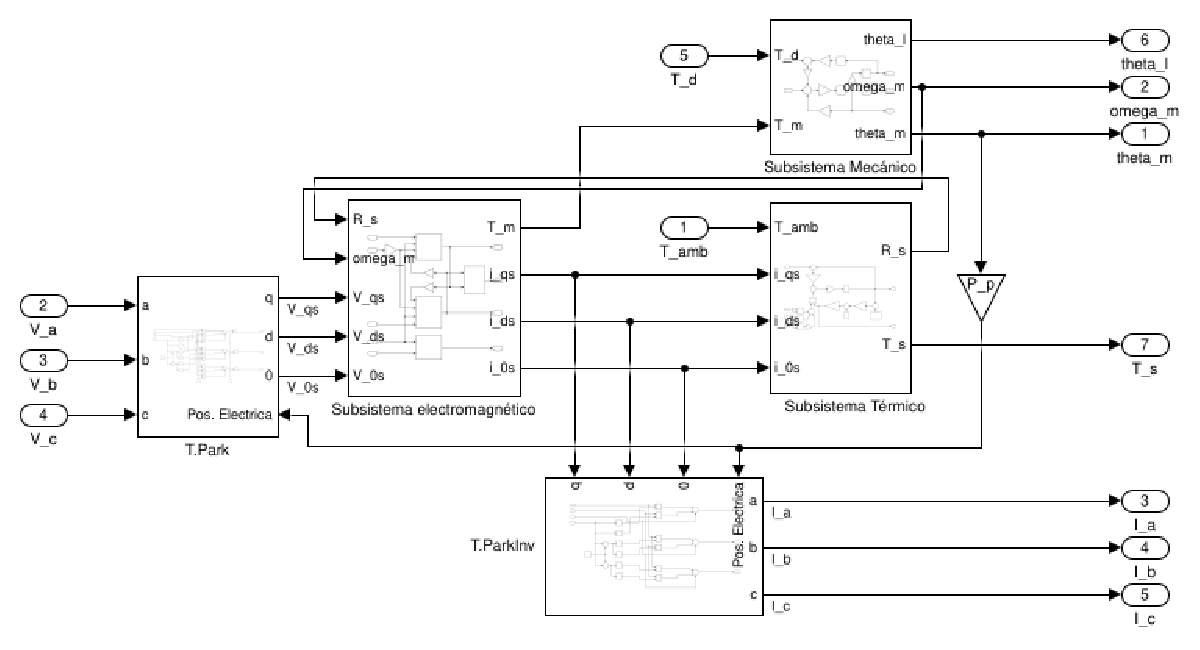
\includegraphics{9-Sistema_Físico_Completo.eps}}
    \end{adjustbox}
    \caption{Diagrama de bloques del sistema físico completo.}
    \label{diagrama de bloques del sistema fisico}
\end{figure}

\begin{figure}[thpb]
    \centering
    \begin{adjustbox}{max width=\columnwidth}
        \framebox{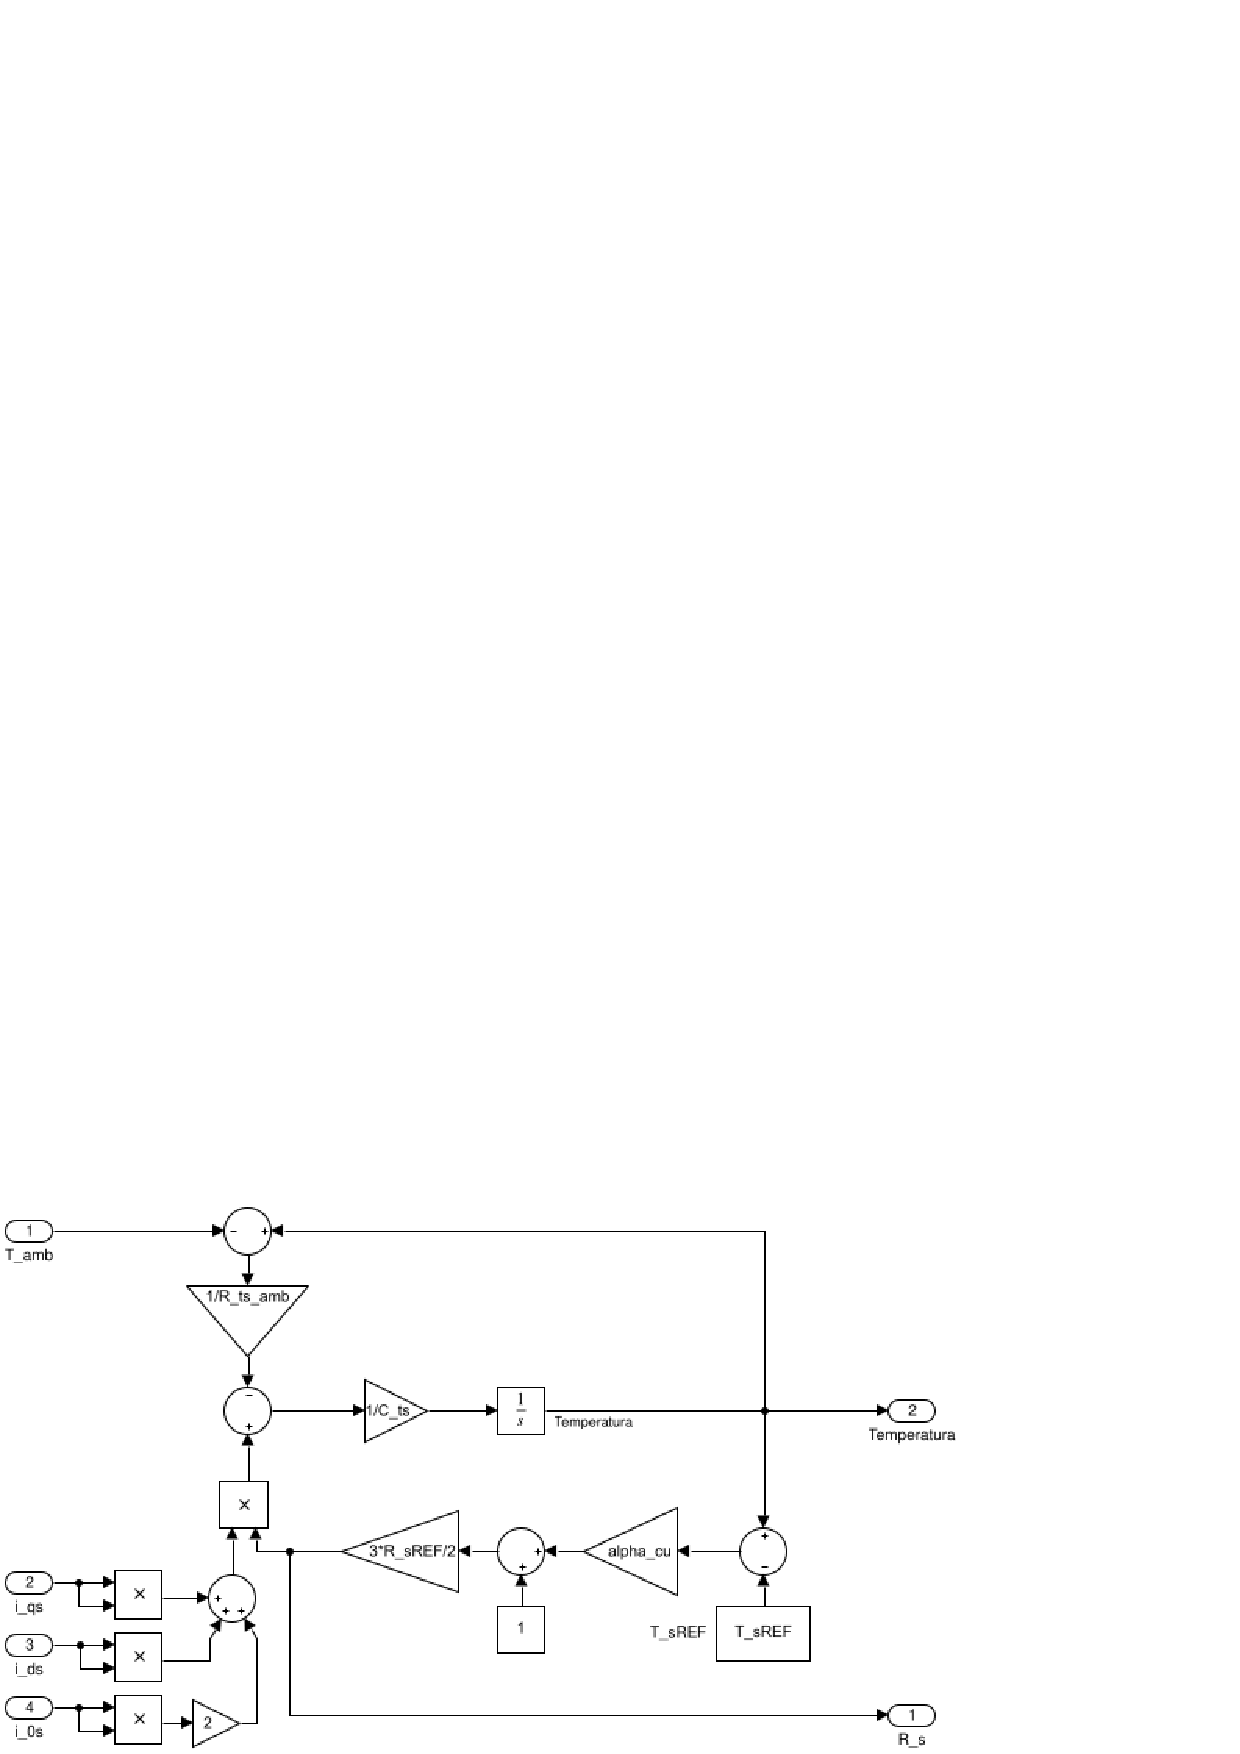
\includegraphics{3-Subsistema_Térmico.png}}
    \end{adjustbox}
    \caption{Diagrama de bloques del sub-sistema térmico}
    \label{subsistema termico}
\end{figure}

\begin{figure}[thpb]
    \centering
    \begin{adjustbox}{max width=\columnwidth}
        \framebox{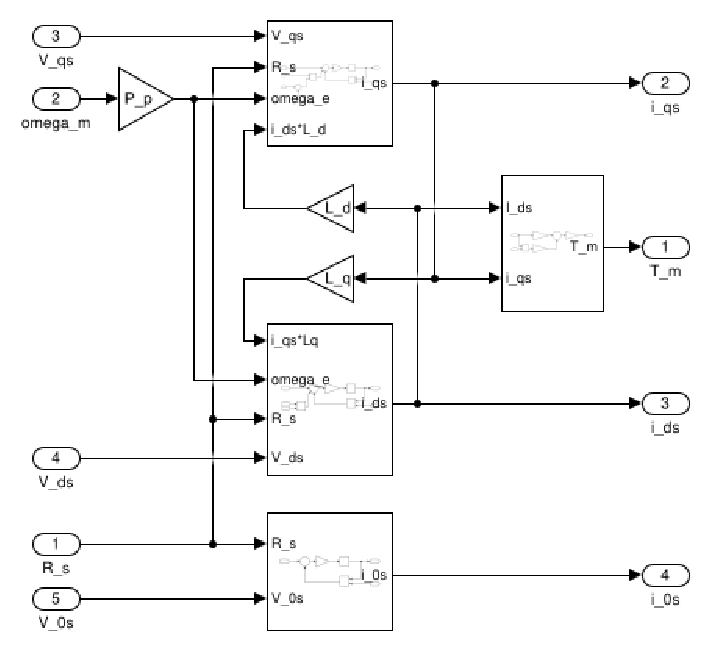
\includegraphics{8-Subsistema_Electromagnético.eps}}
    \end{adjustbox}
    \caption{Diagrama de bloques del sub-sistema electromagnético}
    \label{sub-sistema electromagnetico}
\end{figure}

\begin{figure}[thpb]
    \centering
    \begin{adjustbox}{max width=\columnwidth}
        \framebox{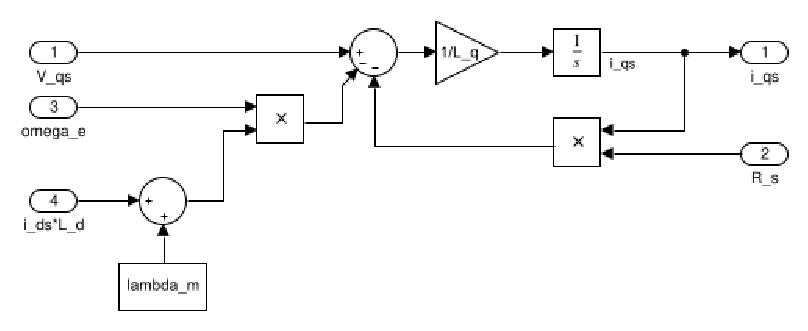
\includegraphics{4-I_qs.eps}}
    \end{adjustbox}
    \caption{Diagrama de bloques $I_{qs}$}
    \label{diagrama de bloques I_qs}
\end{figure}

\begin{figure}[thpb]
    \centering
    \begin{adjustbox}{max width=\columnwidth}
        \framebox{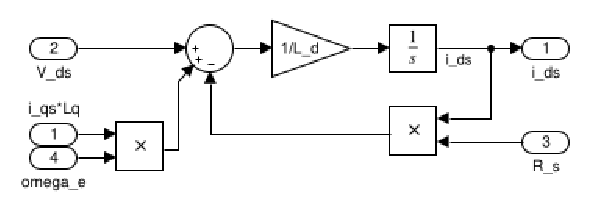
\includegraphics{5-I_ds.eps}}
    \end{adjustbox}
    \caption{Diagrama de bloques $I_{ds}$}
    \label{diagrama de bloques I_ds}
\end{figure}

\begin{figure}[thpb]
    \centering
    \begin{adjustbox}{max width=\columnwidth}
        \framebox{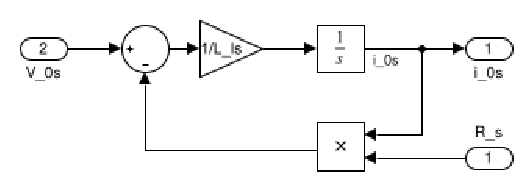
\includegraphics{6-I_0s.eps}}
    \end{adjustbox}
    \caption{Diagrama de bloques $I_{0s}$}
    \label{diagrama de bloques I_0s}
\end{figure}

\begin{figure}[thpb]
    \centering
    \begin{adjustbox}{max width=\columnwidth}
        \framebox{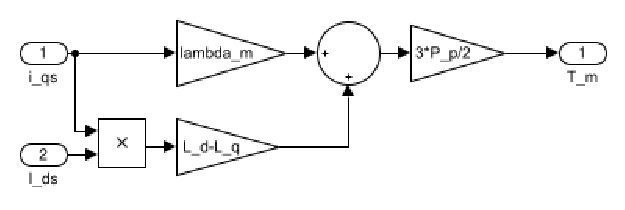
\includegraphics{7-T_m.eps}}
    \end{adjustbox}
    \caption{Diagrama de bloques $T_m$}
    \label{diagrama de bloques T_m}
\end{figure}

\begin{figure}[thpb]
    \centering
    \begin{adjustbox}{max width=\columnwidth}
        \framebox{\includegraphics{10-Transformación_de_Park.eps}}
    \end{adjustbox}
    \caption{Transformación de Park Directa}
    \label{transformacion de Park}
\end{figure}

\begin{figure}[thpb]
    \centering
    \begin{adjustbox}{max width=\columnwidth}
        \framebox{\includegraphics{11-Transformación_de_Park_Inversa.eps}}
    \end{adjustbox}
    \caption{Transformación de Park inversa}
    \label{transformacion de Park inversa}
\end{figure}

% 5.1.1.B Linealización Jacobiana.
\paragraph{\textbf{Linealización Jacobiana}}
Se aclara aquí que, solamente para este ejercicio, se considera un vector de entradas de perturbación modificado
respecto al indicado en \cref{vector de entradas} al considerar $T_l(t)$ desarrollada como se indica en la \cref{torque de carga}.
Lo que se hace es reemplazar $T_l(t)$ por $T_d(t)$ en el vector de la \cref{vector de entradas de perturbacion} lo
cual cambia la definición de $\mathbf{u}(t)$ dada por la \cref{vector de entradas}. Luego, el vector
de entradas de perturbación y el vector de entradas total del sistema, para este ejercicio, son los que se indican en la \cref{vector de entradas jacobi linealizado}.
Cómo se puede observar, se toman las entradas de tensión de control en el espacio de coordenadas $qdo^r$.
\begin{equation}
    \mathbf{u_{d}}(t) = \begin{bmatrix} T_d(t) \\ T_{amb}^{\circ}(t)\end{bmatrix}\, \, \, 
    \mathbf{u}(t) = \begin{bmatrix} v^r_{qs}(t) \\ v^r_{ds}(t) \\ v^r_{0s}(t) \\ T_d(t) \\ T_{amb}^{\circ}(t) \end{bmatrix}
    \label{vector de entradas jacobi linealizado}
\end{equation}

Con esta definición del vector de entradas, la ecuación vectorial de estado del sistema es redefinida.
Por un lado se debe operar para obtener una expresión de $T_l(t)$ en función de $\theta_m(t)$ y no en función de 
$\theta_l(t)$ como se indica en la \cref{torque de carga} para luego reemplazar la expresión obtenida en la \cref{ecuacion vectorial de estado del sistema}.
El procedimiento se indica en \cref{reemplazo de T_l}. Finalmente, la ecuación vectorial de estado del sistema queda expresada
como se indica en la \cref{ecuacion vectorial de estado jacobi}.

\begin{equation}
    \begin{aligned}
        \cref{relacion de velocidad en caja} \,\text{y}\, \cref{velocidad y posición de la carga}\,&\rightarrow\,\theta_l(t) = \frac{1}{r} \int_{0}^{t} \omega_m(\zeta) \, d\zeta + \theta_l(0)\\
        \cref{posicion y velocidad motor}\,&\rightarrow\,  \int_{0}^{t} \omega_m(\zeta) \, d\zeta = \theta_m(t) - \theta_m(0)\\
        \text{Reemplazando la segunda en la primera}\,&\rightarrow\,\theta_l(t) = \frac{\theta_m(t) - \theta_m(0)}{r} + \theta_l(0)\\
        \text{Consideramos que se cumple}\,&\rightarrow\,\frac{\theta_m(0)}{r} = \theta_l(0)\\
        \text{Luego}\,&\rightarrow\,\theta_l(t) = \theta_m(t)/r\\
        \text{Finalmente}\,&\rightarrow\,T_l(t) = k_l\sin\left(\frac{\theta_m(t)}{r}\right) + T_d(t)
    \end{aligned}
    \label{reemplazo de T_l}
\end{equation}

\begin{equation}
    \begin{bmatrix} 
        \frac{d \theta_m(t)}{dt} \\ 
        \frac{d \omega_m(t)}{dt} \\ 
        \frac{d i^r_{qs}(t)}{dt} \\ 
        \frac{d i^r_{ds}(t)}{dt} \\ 
        \frac{d i_{0s}(t)}{dt} \\ 
        \frac{d T^\circ_s(t)}{dt} 
    \end{bmatrix} 
        = 
    \begin{bmatrix} 
        \omega_m(t) \\ 
        \frac{\frac{3}{2} P_p i^r_{qs}(t)\left[\lambda'^r_m + (L_d - L_q) i^r_{ds}(t) \right]}{J_{eq}} - \frac{b_{eq}\omega_m(t)}{J_{eq}} - \frac{k_l\sin\left(\frac{\theta_m(t)}{r}\right)}{rJ_{eq}}\\ 
        -\frac{R_s(t) i^r_{qs}(t)}{L_q} - \frac{P_p \omega_m(t) \left[\lambda'^r_m + L_d i^r_{ds}(t)\right]}{L_q}\\ 
        -\frac{R_s(t) i^r_{ds}(t)}{L_d} + \frac{P_p \omega_m(t) L_q  i^r_{qs}(t)}{L_d}  \\ 
        -\frac{R_s(t) i_{0s}(t) }{L_{ls}} \\ 
        \frac{\frac{3}{2} R_s(t) \left[ i_{qs}^2(t) + i_{ds}^2(t) + 2 i_{0s}^2(t) \right]}{C_{ts}} - \frac{T_s^{\circ}(t)}{R_{ts}C_{ts}}
    \end{bmatrix}
        + 
    \begin{bmatrix} 
        0 & 0 & 0 & 0 & 0 \\ 
        0 & 0 & 0 & \frac{-1}{r J_{eq}} & 0 \\ 
        \frac{1}{L_q} & 0 & 0 & 0 & 0\\ 
        0 & \frac{1}{L_d} & 0 & 0 & 0 \\ 
        0 & 0 & \frac{1}{L_{ls}}  & 0 & 0 \\ 
        0 & 0 & 0 & 0 & \frac{1}{C_{ts} R_{ts}}
    \end{bmatrix} 
    \begin{bmatrix} 
        v^r_{qs}(t) \\ 
        v^r_{ds}(t) \\ 
        v_{0s}(t) \\
        T_d(t) \\ 
        T^{\circ}_{amb}(t)
    \end{bmatrix}
    \label{ecuacion vectorial de estado jacobi}
\end{equation}

En el modelo de pequeñas desviaciones locales $\delta \mathbf{x}(t)$ respecto de los puntos de equilibrio $\mathbf{X}_o(t)$
se hacen las consideraciones señaladas en la \cref{pequeñas desviaciones}.

\begin{equation}
    \begin{cases}
    \mathbf{x}(t)  = \mathbf{X}_o(t) + \mathbf{\delta x}(t)\\
    \mathbf{\delta x}(0) \equiv \mathbf{0}
    \end{cases}
    \label{pequeñas desviaciones}
\end{equation}

Por un lado, la ecuación del \textbf{espacio de operación global NL cuasi-estacionario} se muestra en la \cref{modelo de operacion NL cuasi-estacionario}.

\begin{equation}
    \begin{cases}
    \frac{d\mathbf{X}_o(t)}{dt} =  \mathbf{f}(\mathbf{X}_o(t), \mathbf{U}_o(t)) \approx 0/\text{const};  \mathbf{X}_o(0) \equiv \mathbf{x}_0\\
    \mathbf{Y}_o(t) = C \mathbf{X}_o(t)
    \end{cases}
    \label{modelo de operacion NL cuasi-estacionario}
\end{equation}

Para nuestro sistema queda expresado como se indica en la \cref{modelo de operacion NL cuasi_estacionario desarrollado} para la ecuación de estado.
\begin{equation}
    \begin{bmatrix}
        \frac{d \theta_{m-o}(t)}{dt}\\
        \frac{d \omega_{m-o}(t)}{dt}\\
        \frac{d i^r_{qs-o}(t)}{dt}\\
        \frac{d i^r_{ds-o}(t)}{dt}\\
        \frac{d i_{0s-o}(t)}{dt}\\
        \frac{d T^\circ_{s-o}(t)}{dt}
    \end{bmatrix}
    =
    \begin{cases}
        \omega_{m-o}(t) &\approx \omega_{m0}\\
        \frac{1}{J_{eq}}\left[\frac{3}{2} P_p i^r_{qs-o}(t)\left[\lambda'^r_m + (L_d - L_q) i^r_{ds-o}(t) \right] - b_{eq}\omega_{m-o}(t) - \frac{k_l}{r}\sin\left(\frac{\theta_{m-o}(t)}{r}\right) - \frac{1}{r}T_{d-o}(t)\right] &\approx 0\\
        \frac{1}{L_q}\left[-R_{s-o}(t) i^r_{qs-o}(t)- P_p \omega_{m-o}(t) \left[\lambda'^r_m + L_d i^r_{ds-o}(t)\right] + v^r_{qs-o}(t)\right] &\approx 0\\ 
        \frac{1}{L_d}\left[-R_{s-o}(t) i^r_{ds-o}(t) + P_p \omega_{m-o}(t) L_q  i^r_{qs-o}(t) + v^r_{ds-o}(t)\right] &\approx 0\\ 
        \frac{1}{L_{ls}}\left[-R_{s-o}(t) i_{0s}(t) + v_{0s-o}(t)\right] &\approx 0\\ 
        \frac{3}{2}\frac{R_{s-o}(t)}{C_{ts}} \left[ i_{qs-o}^2(t) + i_{ds-o}^2(t) + 2 i_{0s-o}^2(t) \right] + \frac{1}{R_{ts}C_{ts}}\left[T^{\circ}_{amb-o}(t) - T_{s-o}^{\circ}(t)\right] &\approx 0
    \end{cases}
    \label{modelo de operacion NL cuasi_estacionario desarrollado}
\end{equation}

Las condiciones
iniciales se señalan en la \cref{condiciones inciales cuasi-estacionario}.

\begin{equation}
    \mathbf{X_o}(0)
    =
    \begin{bmatrix} 
        \theta_{m-o}(0) \\ 
        \omega_{m-o}(0) \\ 
        i^r_{qs-o}(0) \\ 
        i^r_{ds-o}(0)\\ 
        i_{0s-o}(0)\\ 
        T^\circ_{s-o}(0)
    \end{bmatrix}
    =
    \begin{bmatrix} 
        \theta_{m0} \\ 
        \omega_{m0} \\ 
        i^r_{qs0} \\ 
        i^r_{ds0} \\ 
        i_{0s0} \\ 
        T^\circ_{s0} 
    \end{bmatrix}
    \label{condiciones inciales cuasi-estacionario}
\end{equation}

En las \cref{modelo de operacion NL cuasi_estacionario desarrollado} y \cref{condiciones inciales cuasi-estacionario}
el sub-índice $-o$ indica los valores de las variables en el punto de operación.

Consideramos relevante hacer aquí un análisis al respecto
del espacio de operación global NL para estem modelo del sistema físico
en particular.

Si en lugar de la restricción débil señalada en la primera ecuación de la \cref{modelo de operacion NL cuasi-estacionario}
se toma la restricción fuerte dada por la \cref{restriccion fuerte}. Tendremos un
punto de operación definido como en la \cref{punto de operacion} tomando en cuenta
las condiciones iniciales del modelo señaladas en \cref{modelo de operacion NL cuasi_estacionario desarrollado} y 
la evolución de $\theta_m(t)$ dada por la \cref{posicion y velocidad motor}.


\begin{equation}
    \frac{d\mathbf{X}_o(t)}{dt} =  \mathbf{f}(\mathbf{X}_o(t), \mathbf{U}_o(t)) \equiv 0/\text{const}
    \label{restriccion fuerte}
\end{equation}

\begin{equation}
    \mathbf{X_o}(t)
    =
    \begin{bmatrix} 
        \theta_{m-o}(t) \\ 
        \omega_{m-o}(t) \\ 
        i^r_{qs-o}(t) \\ 
        i^r_{ds-o}(t)\\ 
        i_{0s-o}(t)\\ 
        T^\circ_{s-o}(t)
    \end{bmatrix}
    =
    \begin{bmatrix} 
        \int_{0}^{t} \omega_{m-o}(0) d\tau + \theta_{m-o}(0)\\
        \omega_{m-o}(0)\\
        i^r_{qs-o}(0) \\
        i^r_{ds-o}(0)\\
        i_{0s-o}(0)\\
        T^\circ_{s-o}(0)
    \end{bmatrix}
    =
    \begin{bmatrix} 
        \omega_{m0}t + \theta_{m0}\\
        \omega_{m0} \\ 
        i^r_{qs0} \\ 
        i^r_{ds0} \\ 
        i_{0s0} \\ 
        T^\circ_{s0} 
    \end{bmatrix}
    \label{punto de operacion}
\end{equation}

Reemplazamos lo obtenido en \cref{punto de operacion} en la \cref{modelo de operacion NL cuasi_estacionario desarrollado}
y destacamos la ecuación de estado asociada a $\omega_(t)$.

\begin{equation}    
    \frac{1}{J_{eq}}\left[\frac{3}{2} P_p i^r_{qs0}\left[\lambda'^r_m + (L_d - L_q) i^r_{ds0} \right] - b_{eq}\omega_{m0} - \frac{k_l}{r}\sin\left(\frac{\omega_{m0}t + \theta_{m0}}{r}\right) - \frac{1}{r}T_{d0}\right] = 0
    \label{ecuacion de estado omega_m espacio NL de operacion}
\end{equation}

Se puede ver en la \cref{ecuacion de estado omega_m espacio NL de operacion} que 
existe una dependencia explícita de $t$, no solamente de las variables de 
estado y de las entradas en el punto de operación. Al considerar
un punto de operación cuasiestacionario, la \cref{ecuacion de estado omega_m espacio NL de operacion}
se puede expresar de forma simplificada, para mostrar nuestro punto, como en la \cref{ecuacion de estado omega_m espacio NL de operacion simplificada}.

\begin{equation}    
    cte - \frac{k_l}{r}\sin\left(\frac{\omega_{m0}t + \theta_{m0}}{r}\right) - \frac{1}{r}T_{d-o}(t) = 0
    \label{ecuacion de estado omega_m espacio NL de operacion simplificada}
\end{equation}

Condición que se puede satisfacer solo bajo dos supuestos distintos indicados en la \cref{condiciones de satisfaccion}.
La primera de ellas implica tener control sobre la entrada de perturbación $T_{d-o}$, lo cual
no es posible por definición, o bién si se tuviera un contrapeso que equilibre el torque
gravitacional producido por el brazo y la masa que transporta en su extremo. La segunda condición
elimina la dependencia explícita de $t$ y no requiere control sobre la entrada de perturbación para
lograrse.

\begin{equation}
    \begin{cases}
        T_{d-o}(t) = cte - \frac{k_l}{r}\sin\left(\frac{\omega_{m0}t + \theta_{m0}}{r}\right)\\
        \omega_{m0} = 0
    \end{cases}
    \label{condiciones de satisfaccion}
\end{equation}

Cuando se asume la segunda condición de la \cref{condiciones de satisfaccion},
la \cref{modelo de operacion NL cuasi_estacionario desarrollado} queda como se indica en la 
\cref{modelo de operacion NL cuasi_estacionario desarrollado reducido}. En la que
además se toma $v_{0s-o}(t) \equiv 0$ al tratarse de un sistema de
tensiones trifásico simétrico balanceado. Eso da por resultado $i_{ds0} = 0$,
al ser $R_{s-o} \neq 0$ para las temperaturas normales de operación, y se reemplaza directamente en la 
ecuación de estado de la $T^{\circ}_{s}$.

\begin{equation}
    \begin{cases}
        \omega_{m0} &= 0\\
        \frac{1}{J_{eq}}\left[\frac{3}{2} P_p i^r_{qs0}\left[\lambda'^r_m + (L_d - L_q) i^r_{ds0} \right] - \frac{k_l}{r}\sin\left(\frac{\theta_{m0}}{r}\right) - \frac{1}{r}T_{d-o}\right] &= 0\\
        \frac{1}{L_q}\left[-R_{s-o} i^r_{qs0} + v^r_{qs-o}\right] &= 0 \Rightarrow i^r_{qs0} = v^r_{qs-o}/R_{s-o}\\ 
        \frac{1}{L_d}\left[-R_{s-o} i^r_{ds0} + v^r_{ds-o}\right] &= 0 \Rightarrow i^r_{ds0} = v^r_{ds-o}/R_{s-o}\\ 
        \frac{1}{L_{ls}}\left[-R_{s-o} i_{0s}\right] &= 0 \Rightarrow i_{0s} = 0\\ 
        \frac{3}{2}\frac{R_{s-o}}{C_{ts}} \left[ i_{qs0}^2+ i_{ds0}^2 \right] + \frac{1}{R_{ts}C_{ts}}\left[T^{\circ}_{amb-o} - T_{s0}^{\circ}\right] &= 0
    \end{cases}
    \label{modelo de operacion NL cuasi_estacionario desarrollado reducido}
\end{equation}

Presentamos aquí las curvas que permitan obtener las entradas
de control que es necesario aplicar para obtener una posición
del brazo, dado un vector de entradas de perturbación constantes.

En \cref{T_m en función de la posición y T_do} representamos
el $T_{m-o}$ que se requiere para una preturbación $T_{d-o}$ dada,
en función de la posición del brazo. En donde se
consideran los valores extremos de $T_{d-o}$ y un
un valor de $k_l = 9.807 \left[N.m\right]$, ambos en los rangos
dados en \cite{c1}.

\begin{figure}[thpb]
    \centering
    \begin{adjustbox}{scale = 0.6}
        \framebox{\includegraphics{14-T_m_vs_thetha_vd_Td.pdf}}
    \end{adjustbox}
    \caption{$T_m$ respecto a $T_{d-o}$ y $\theta_l$}
    \label{T_m en función de la posición y T_do}
\end{figure}

Luego, dado un valor de corriente total junto con un
ángulo $\beta$ como se indica en la \cref{corriente total}, y que se pueden relacionar
gráficamente como en la \cref{restriccion de corriente maxima}, podemos expresar
las curvas de $T_{m-o}$ en función de $i^{r}_{qd0s-o}$ con $\beta$ como parametro, las que
se muestran en la \cref{T_m respecto a i_qd0s-o} y que responden a la \cref{ecuación T_m respecto a i_qd0s-o}.


\begin{equation}
    \left(i^{r}_{qd0s-o}\right)^2 = \left(i^{r}_{qs0}\right)^2 + \left(i^{r}_{ds0}\right)^2
    \label{corriente total}
\end{equation}

\begin{equation}
    \frac{3}{2} P_p i^r_{qd0s-o}\sin(\beta)\left[\lambda'^r_m + (L_d - L_q) i^r_{qd0s-o}\cos(\beta)\right]
    \label{ecuación T_m respecto a i_qd0s-o}
\end{equation}

\begin{figure}[thpb]
    \centering
    \begin{adjustbox}{scale = 0.6}
        \framebox{\includegraphics{15-Circulos_de_corriente.pdf}}
    \end{adjustbox}
    \caption{circulos de corriente total en coordenadas virtuales.}
    \label{restriccion de corriente maxima}
\end{figure}

\begin{figure}[thpb]
    \centering
    \begin{adjustbox}{scale = 0.6}
        \framebox{\includegraphics{17-T_m_vs_corriente_vs_beta.pdf}}
    \end{adjustbox}
    \caption{$T_m$ respecto de $i^r_{qd0s-o}$ con parámetro $\beta$.}
    \label{T_m respecto a i_qd0s-o}
\end{figure}

De la última ecuación en la \cref{modelo de operacion NL cuasi_estacionario desarrollado reducido}
se puede obtener $T^{\circ}_{s0}$ a partir del conocimiento de la corriente total. Esto se expresa en la
\cref{T_s respecto a la corriente total} y da como resultado la gráfica mostrada en \cref{grafica T_s respecto a la corriente} en donde
se grafica la $T^{\circ}_{s0}$ respecto a $i^{r}_{qd0s-o}$ con $T^{\circ}_{amb-o}$ como parámetro.

\begin{equation}
    T^{\circ}_{s0} = \frac{\frac{3}{2}R_{sREF}\left(\alpha_{cu}T^{\circ}_{sREF} - 1\right)\left(i^{r}_{qd0s-o}\right)^2 - \frac{T^{\circ}_{amb-o}}{R_{ts-amb}}}{\frac{3}{2}R_{sREF}\alpha_{cu}\left(i^{r}_{qd0s-o}\right)^2 - \frac{1}{R_{ts-amb}}}
    \label{T_s respecto a la corriente total}
\end{equation}

\begin{figure}[thpb]
    \centering
    \begin{adjustbox}{scale = 0.6}
        \framebox{\includegraphics{16-Temperatura_vs_corriente.pdf}}
    \end{adjustbox}
    \caption{$T^{\circ}_s$ respecto de $i^r_{qd0s-o}$ con parámetro $T^{\circ}_{amb}$.}
    \label{grafica T_s respecto a la corriente}
\end{figure}

Por otro lado, el \textbf{Modelo dinámico LPV} se indica en la \cref{modelo de pequeñas desviaciones}:

\begin{equation}
    \begin{cases}
        \frac{d}{dt} \mathbf{\delta x}(t) \approx A(t) \mathbf{\delta x}(t) + B(t) \mathbf{\delta u}(t); \mathbf{\delta x}(0) \equiv \mathbf{0}\\
        \mathbf{\delta y}(t) = C\mathbf{\delta x}(t)
    \end{cases}
    \label{modelo de pequeñas desviaciones}
\end{equation}

Las matrices $A(t)$ y $B(t)$ de la \cref{modelo de pequeñas desviaciones} vienen dadas por la \cref{matriz_AB}.

\begin{equation}
    A(t) = \left[ \left. \frac{\mathbf{\partial f}}{\mathbf{\partial x}} \right|_{o}(t) \right] =
    \begin{bmatrix}
        \frac{\partial}{\partial x}\left( \frac{d \theta_m(t)}{dt}\right) \\ 
        \frac{\partial}{\partial x}\left( \frac{d \omega_m(t)}{dt}\right) \\
        \frac{\partial}{\partial x}\left( \frac{d i^r_{qs}(t)}{dt}\right) \\ 
        \frac{\partial}{\partial x}\left( \frac{d i^r_{ds}(t)}{dt}\right) \\ 
        \frac{\partial}{\partial x}\left( \frac{d i^r_{0s}(t)}{dt}\right) \\ 
        \frac{\partial}{\partial x}\left( \frac{d T^\circ_s(t)}{dt}\right) 
    \end{bmatrix}\quad
    B(t) = \left[ \left. \frac{\mathbf{\partial f}}{\mathbf{\partial u}} \right|_{o}(t) \right] =
    \begin{bmatrix}
        0 & 0 & 0 & 0 & 0\\
        0 & 0 & 0 & \frac{-1}{r J_{eq}} & 0\\
        \frac{1}{L_q} & 0 & 0 & 0 & 0\\
        0 & \frac{1}{L_d} & 0 & 0 & 0\\
        0 & 0 & \frac{1}{L_d} & 0 & 0\\
        0 & 0 & 0 & 0 & \frac{1}{C_{ts} R_{ts}}
    \end{bmatrix}
    \label{matriz_AB}
\end{equation}

Los gradientes indicados para $A(t)$ en la \cref{matriz_AB} vienen dados por la \cref{gradientesA}.

\begin{equation}
    \begin{aligned}
        \frac{\partial}{\partial x}\left( \frac{d \theta_m(t)}{dt}\right) &= \begin{bmatrix} 0 & 1 & 0 & 0 & 0 & 0 \end{bmatrix}\\
        \frac{\partial}{\partial x}\left( \frac{d \omega_m(t)}{dt}\right) &= \begin{bmatrix}
        \frac{-K_{l} \cos\left(\frac{\theta_m(t)}{r}\right)}{J_{eq} r^2} & \frac{-b_{eq}}{J_{eq}} & \frac{3 P_p \left(\lambda_m+i^r_{ds}(t) \left(L_d-L_q\right)\right)}{2 J_{eq}} & \frac{3 P_p i^r_{qs}(t) \left(L_d-L_q\right)}{2 J_{eq}} & 0 & 0 
        \end{bmatrix}\\
        \frac{\partial}{\partial x}\left( \frac{d i^r_{qs}(t)}{dt}\right) &= \begin{bmatrix} 
        0 & \frac{-3 P_p \left(i^r_{ds}(t) L_d+\lambda_m\right)}{2 L_q} & \frac{-R_s(t)}{L_q} & \frac{-L_d P_p \omega_m(t)}{L_q} & 0 & \frac{-R_{sREF} \alpha_{cu} i^r_{qs}(t)}{L_q} 
        \end{bmatrix}\\
        \frac{\partial}{\partial x}\left( \frac{d i^r_{ds}(t)}{dt}\right) &= \begin{bmatrix} 
        0 & \frac{L_q P_p i^r_{qs}(t)}{L_d} & \frac{L_q P_p \omega_m(t)}{L_d} & \frac{-R_s(t)}{L_d} & 0 & \frac{-R_{sREF} \alpha_{cu} i^r_{ds}(t)}{L_d} 
        \end{bmatrix}\\
        \frac{\partial}{\partial x}\left( \frac{d i_{0s}(t)}{dt}\right) &= \begin{bmatrix} 
        0 & 0 & 0 & 0 & \frac{-R_s(t)}{L_{ls}} & \frac{-R_{sREF} \alpha_{cu} i_{0s}(t)}{L_{ls}} 
        \end{bmatrix}\\
        \frac{\partial}{\partial x}\left( \frac{d T^\circ_s(t)}{dt}\right) &= \begin{bmatrix} 
        0 & 0 & \frac{3 R_s(t) i^r_{qs}(t)}{C_{ts}} & \frac{3 R_s(t) i^r_{ds}(t)}{C_{ts}} & \frac{6 R_s(t) i^r_{0s}(t)}{C_{ts}} & \frac{3 R_{sREF} \alpha_{cu} \left({i^r_{ds}(t)}^2+2 {i^r_{0s}(t)}^2+{i^r_{qs}(t)}^2\right)}{2 C_{ts}} - \frac{1}{C_{ts} R_{ts}} 
        \end{bmatrix}\\
    \end{aligned}
    \label{gradientesA}
\end{equation}

Nota: Por motivos de legibilidad del modelo matemático LPV completo, decidimos conservar la expresión en esta forma desagregada.

\paragraph{\textbf{Linealización Por Realimentación No Lineal}}
Dado que la dinámica del sub-sistema térmico es comparativamente
más lenta que la dinámica del resto del sistema físico, lo que da por resultado
una variación relativamente lenta de la $T_s(t)$ y por lo tanto de la $R_s(t)$,
en este análisis no se tendrá en cuenta el acoplamiento no lineal con el sub-sistema térmico (el que se da a través de la $R_s(t)$), 
pero si se considerará su dinámica lineal. Además, teniendo en cuenta que el sistema de tensiones $v_{abcs}(t)$ es un sistema
simétrico balanceado, podemos asumir primero $v_{0s}(t) \equiv 0$, lo que da por resultado $i_{0s}(t) \equiv 0$ en estado permanente. Esto sumado a la especificación $i^{r}_{ds}(t)\equiv0$, 
la que imponemos directamente, hace que se pueda considerar para el análisis, un vector de estado reducido dado por \cref{vector de estado reducido}.

\begin{equation}
    \mathbf{x}(t) = \begin{bmatrix} \theta_m(t) \\ \omega_m(t) \\ i^r_{qs}(t)\end{bmatrix}
    \label{vector de estado reducido}
\end{equation}

Las ecuaciones de estado resultantes se indican en la \cref{ecuacion con ids=0}.
En la que se puede observar que se toma $R_s$ constante en lugar  de $R_s(t)$ al
no considerar el acoplamiento con el sub-sistema térmico.

\begin{equation}
	\begin{cases}
		\frac{d \theta_m(t)}{dt}  &= {\omega}_m(t)\\
		\frac{d \omega_m(t)}{dt}  &= \frac{3}{2} \frac{P_p i^r_{qs}(t)\lambda^r_m}{J_{eq}} - \frac{b_{eq}\omega_m(t)}{J_{eq}} - \frac{T_l(t)}{r J_{eq}}\\
		\frac{d i^r_{qs}(t)}{dt}  &= -\frac{R_s i^r_{qs}(t)}{L_q} - \frac{P_p \omega_m(t) \lambda^r_m}{L_q}+ \frac{v^r_{qs}(t)}{L_q}
    \end{cases}
	\label{ecuacion con ids=0}
\end{equation}

Expresándolo en forma de espacio de estados se obtienen las
\textbf{ecuaciones matriciales LTI de estado y de salida (con estado inicial genérico)}
como se indica en \cref{ecuacion matricial con ids=0}.

\begin{equation}
	\begin{cases}
		\begin{bmatrix}
			\frac{d \theta_m(t)}{dt} \\ 
			\frac{d \omega_m(t)}{dt}\\
			\frac{d i^r_{qs}(t)}{dt}  
		\end{bmatrix}
		 = 
		 \begin{bmatrix}
		 	0 & 1 & 0 & 0& 0\\ 
		 	0 & - \frac{b_{eq}}{J_{eq}} & \frac{3}{2} \frac{P_p \lambda^r_m}{J_{eq}}& 0 & 0\\
		 	0 &  - \frac{P_p  \lambda^r_m}{L_q} & -\frac{R_s}{L_q} & 0 & 0\\
            0 & \frac{P_p \omega_m(t) L_q i^r_{qs}(t)}{L_d}
		 \end{bmatrix}
		 \begin{bmatrix}
		 	{\theta}_m(t) \\ 
		 	{\omega}_m(t)\\
		 	{i}^r_{qs}(t)  
		 \end{bmatrix}
		 +
		 \begin{bmatrix}
		 	0 \\ 
		 	0\\
		 	\frac{1}{L_q}  
		 \end{bmatrix}
		 v^r_{qs}(t)+
		 \begin{bmatrix}
		 	0 \\ 
		 	- \frac{1}{r J_{eq}}\\
		 	0 
		 \end{bmatrix} T_l(t)\,\,; \mathbf{x}(0) = \mathbf{x_0}\\
		 y(t) = \begin{bmatrix}
		 		1 & 0 & 0
		 	 \end{bmatrix}
		 	 \begin{bmatrix}
		 	 	{\theta}_m(t) \\ 
		 	 	{\omega}_m(t)\\
		 	 	{i}^r_{qs}(t)
		 	 \end{bmatrix}
	\end{cases}
	\label{ecuacion matricial con ids=0}
\end{equation}

La dinámica resultante del sub-sistema térmico,
indicada en la \cref{dinamica sub-sistema térmico},
se obtiene al reemplazar en la ecuación de estado de la $T^{\circ}_s$
(\cref{ecuacion vectorial de estado del sistema}) las consideraciones indicadas al inicio de este inciso al
respecto de las corrientes. En la misma, el término $\frac{3}{2}\frac{R_{s}}{C_{ts}} i_{qs}^2(t)$ representa
la $P_{perd}(t)$, que al considerarse como entrada junto con la $T^{\circ}_{amb}(t)$ ponen de
manifiesto la dinámica lineal indicada.

\begin{equation}
    \frac{d T^\circ_{s}(t)}{dt} = \frac{3}{2}\frac{R_{s}}{C_{ts}} i_{qs}^2(t) + \frac{1}{R_{ts}C_{ts}}\left[T^{\circ}_{amb}(t) - T_{s}^{\circ}(t)\right]
    \label{dinamica sub-sistema térmico}
\end{equation}

El \textbf{diagrama de bloques de estado del LTI equivalente en forma desagregada}, junto con la
dinámica de la $T^{\circ}_s(t)$, se puede observar en la \cref{diagrama de bloques LTI equivalente}. Mientras
que en la \cref{diagrama de bloques LTI equivalente i0s e ids} se muestra la dinámica de la
$i^r_{ds}(t)$ y la $i_{0s}(t)$ bajo las especificaciones indicadas.

\begin{figure}[thpb]
    \centering
    \begin{adjustbox}{max width=\columnwidth}
        \framebox{\includegraphics{18-Diagrama_de_bloques_LTI_equivalente_aumentado.png}}
    \end{adjustbox}
    \caption{Diagrama de bloques LTI equivalente.}
    \label{diagrama de bloques LTI equivalente}
\end{figure}

\begin{figure}[thpb]
    \centering
    \begin{adjustbox}{max width=\columnwidth}
        \framebox{\includegraphics{19-Diagrama_de_bloques_LTI_equivalente_aumentado_i0s_ids.png}}
    \end{adjustbox}
    \caption{Dinámica de $i^r_{ds}(t)$ e $i_{0s}(t)$.}
    \label{diagrama de bloques LTI equivalente i0s e ids}
\end{figure}

Para lograr la especificación indicada para $i^r_{ds}(t)$ es necesario realizar una \textbf{Ley de control mínima} que se determina a partir de la ecuación de estado para $i^{r}_{ds}(t)$ (\cref{ecuacion de estado ids}), partiendo de la hipótesis de que $i^{r}_{ds}(0)=0$:

\begin{equation}
	0= \frac{L_q P_p \omega_m(t)i^r_{qs}(t)}{L_d}  + \frac{v^r_{ds}(t)}{L_d}\Rightarrow	v^{r}_{ds}= -L_{q}i^{r}_{qs}(t)P_{p}\omega_{m}(t)\\
	\label{ecuacion determinacion ley de control minima}
\end{equation}

De esta manera queda determinada la ley de control mínima, que debe aplicarse para lograr el desacoplamiento de los canales de flujo magnético y torque.

La \textbf{Implementación}, en el modelo global NL completo, de esta  ley de control mínima, mediante un controlador parcial incorporando el inversor (modulador de tensión trifásico equivalente), las Transformaciones de Park y los sensores de realimentación ideal de variables de estado,
se puede observar en la \cref{Implementación de ley de control mínima}

\begin{figure}[thpb]
	\centering
	\begin{adjustbox}{max width=\columnwidth}
		\framebox{\includegraphics{12-Ley_de_control_minima}}
	\end{adjustbox}
	\caption{Implementación de ley de control mínima}
	\label{Implementación de ley de control mínima}
\end{figure}

Para el caso general en donde no se cumple la hipótesis $i^{r}_{ds}(0)=0$, existe una \textbf{dinámica residual} en la corriente $i^{r}_{ds}(t)$. Esta dinámica queda representada con la ecuación diferencial que obtenemos al reemplazar la ley de control mínima (\cref{ecuacion determinacion ley de control minima}) en la \cref{ecuacion de estado ids}:

\begin{equation}
	\frac{d i^r_{ds}(t)}{dt} = -\frac{R_s i^r_{ds}(t)}{L_d} \Rightarrow L_d\frac{d i^r_{ds}(t)}{dt} + R_s i^r_{ds}(t) = 0
	\label{ecuacion dinamica residual ids}
\end{equation}

La cual tiene la siguiente solución:

\begin{equation}
	{i}^r_{ds}(t) = {i}^r_{ds}(0) e^{-\dfrac{R_s}{L_d}t} 
\end{equation}

Como se puede observar  si $i^{r}_{ds}(0)\neq0$, ésta decae exponencialmente hasta llegar a 0. Esto establece un acoplamiento con el eje $q$, produciendo un comportamiento no lineal, que se termina desvaneciendo con el tiempo a medida que $i^{r}_{ds}(t)$ decae. Por lo tanto este fenómeno puede ser despreciado para régimen forzado.

Para evitar esto, se puede implementar una \textbf{ley de control complementaria mínima} sobre el eje $q$, y poder eliminar completamente el acoplamiento residual NL, obteniendo así un modelo equivalente lineal del sistema, aún cuando $i^{r}_{ds}(0)\neq0$. Esto se logró implementando una ley de control que permita deshacerse del término que contiene a $i^{r}_{ds}(t)$ en la \cref{ecuacion de estado iqs}.

\begin{align}
	v^r_{qs}(t) &= L_q\frac{d i^r_{qs}(t)}{dt} + R_s i^r_{qs}(t) +P_p \omega_m(t) \lambda'^r_m +\underline{P_p \omega_m(t) L_d i^r_{ds}(t)} \label{ley de control complementaria 1 }\\
	v^r_{qs}(t) &= v^r_{qs}(t)^{*} + P_p \omega_m(t) L_d i^r_{ds}(t)  \label{ley de control complementaria 2}\\
 	v^r_{qs}(t)^{*} &= L_q\frac{d i^r_{qs}(t)}{dt} + R_s i^r_{qs}(t) +P_p \omega_m(t) \lambda'^r_m  \label{ley de control complementaria 3}
\end{align}

\begin{figure}[thpb]
	\centering
	\begin{adjustbox}{max width=\columnwidth}
		\framebox{\includegraphics{13-Ley_de_control_complementaria}}
	\end{adjustbox}
	\caption{Implementación de ley de control complementaria}
	\label{Implementación de ley de control complementaria}
\end{figure}

El modelo \textbf{LTI equivalente(incorporando la dinámica residual del eje $\mathbf{d}$)} queda como se indica en la \cref{equaciones modelo LTI eq} y en la \cref{diagrama de bloques modelo LTI eq}:

\begin{equation}
	\begin{cases}
		\frac{d \theta_m(t)}{dt} = {\omega}_m(t)\\
		\frac{d \omega_m(t)}{dt} = \frac{3}{2} \frac{P_p i^r_{qs}(t)\lambda^r_m}{J_{eq}} - \frac{b_{eq}\omega_m(t)}{J_{eq}} - \frac{T_l(t)}{r J_{eq}}\\
		\frac{d i^r_{qs}(t)}{dt} = -\frac{R_s i^r_{qs}(t)}{L_q} - \frac{P_p \omega_m(t) \lambda^r_m}{L_q}+ \frac{v^r_{qs}(t)}{L_q}\\
		\frac{d i^r_{ds}(t)}{dt} = -\frac{R_s i^r_{ds}(t)}{L_d}	
	\end{cases}
	\label{equaciones modelo LTI eq}
\end{equation}

\begin{figure}[thpb]
	\centering
	\begin{adjustbox}{max width=\columnwidth}
		\framebox{\includegraphics{20-Diagrama_de_bloques_LTI_equivalente_dinamica_residual.png}}
	\end{adjustbox}
	\caption{Diagrama de bloques LTI con dinámica residual eje d}
	\label{diagrama de bloques modelo LTI eq}
\end{figure}

\paragraph{\textbf{Comparación del modelo dinámico LTI equivalente aumentado vs. el modelo dinámico global LPV}}

\paragraph{\textbf{Funciones de Transferencia}}
para el modelo LTI equivalente aumentado, desde ambas entradas $V^r_{qs}(s)$ y $T_l(s)$ hacia la salida ${\Theta}_m(s)$.

Primero se aplicó la Transformada de Laplace a la ecuaciones del sistema LTI equivalente aumentado, considerando condiciones iniciales nulas:

\begin{equation}
	\begin{cases}
		s{\Theta}_m(s) = {\Omega}_m(s)\\
		s{\Omega}_m(s) = \frac{3}{2} \frac{P_p I^r_{qs}(s)\lambda^r_m}{J_{eq}} - \frac{b_{eq}\Omega_m(s)}{J_{eq}} - \frac{T_l(s)}{r J_{eq}}\\
		s{I}^r_{qs}(s) = -\frac{R_s I^r_{qs}(s)}{L_q} - \frac{P_p \Omega_m(s) \lambda^r_m}{L_q}+ \frac{V^r_{qs}(s)}{L_q}	
	\end{cases}
	\label{equaciones modelo LTI eq en s}
\end{equation}

Luego se despejó la salida en función de las entradas, para obtener finalmente las funciones de transferencia:
\begin{align}
	{\Theta}_m(s) &= -\frac{R_{s} \frac{T_l(s)}{r} + L_{q} \frac{T_l(s)}{r} s - \dfrac{3}{2} P_{p} V^r_{qs}(s) \lambda^r_m}{J_{eq} L_{q} s^3 +\left( J_{eq} R_{s} + L_{q} b_{eq} \right)s^2 + \left( R_{s} b_{eq} + \dfrac{3}{2} {P_{p}}^2 { \lambda^r_m}^2\right) s}\label{posicion en funcion de demas variables en laplace}\\
	G_{V^r_{qs}}(s) &= \frac{{\Theta}_m(s)}{V^r_{qs}(s)} = \frac{\dfrac{3}{2} P_{p} \lambda^r_m}{J_{eq} L_{q} s^3 +\left( J_{eq} R_{s} + L_{q} b_{eq} \right)s^2 + \left( R_{s} b_{eq} + \dfrac{3}{2} {P_{p}}^2 { \lambda^r_m}^2\right) s}\label{funcion de transferencia desde Vqs}\\
	G_{T_l}(s) &= \frac{{\Theta}_m(s)}{T_l(s)} = -\frac{\frac{1}{r}\left( R_{s} + L_{q} s\right) }{J_{eq} L_{q} s^3 +\left( J_{eq} R_{s} + L_{q} b_{eq} \right)s^2 + \left( R_{s} b_{eq} + \dfrac{3}{2} {P_{p}}^2 { \lambda^r_m}^2\right) s}
	\label{funcion de transferencia desde T_l}
\end{align}

\subsubsection{\textbf{Análisis de estabilidad a lazo abierto para el modelo LTI equivalente aumentado}}
\paragraph{\textbf{Determinación de polos y ceros del sistema}}
Para determinar los polos, se resolvió el polinomio característico del sistema.

\begin{align}
	J_{eq} L_{q} s^3 +\left( J_{eq} R_{s} + L_{q} b_{eq} \right)s^2 + \left( R_{s} b_{eq} + \dfrac{3}{2} {P_{p}}^2 { \lambda^r_m}^2\right) s = 0 \label{polinomio caracteristico del sistema LTI}\\
\end{align}

Cuyas soluciones fueron:
\begin{equation}
	\begin{cases}
		s_1 = 0\\
		s_2 = \frac{-\left( L_{q} b_{eq} + J_{eq} R_{s}\right)  + \sqrt{{J_{eq}}^2 {R_{s}}^2 - 6 J_{eq} L_{q} {P_{p}}^2 {\lambda^r_m}^2 - 2 J_{eq} L_{q} R_{s} b_{eq}+{L_{q}}^2 {b_{eq}}^2} }{2 J_{eq} L_{q}}\\
		s_3 = \frac{-\left( L_{q} b_{eq} + J_{eq} R_{s}\right)  - \sqrt{{J_{eq}}^2 {R_{s}}^2 - 6 J_{eq} L_{q} {P_{p}}^2 {\lambda^r_m}^2 - 2 J_{eq} L_{q} R_{s} b_{eq}+{L_{q}}^2 {b_{eq}}^2} }{2 J_{eq} L_{q}}
	\end{cases}\label{polos del sistema LTI}
\end{equation}

Además, se obtuvieron las frecuencias naturales y relaciones de amortiguamiento, al comparar la ecuación características asociada a los dos polos complejos conjugados, con  la ecuación estándar de un sistema de segundo orden.

\begin{align}
	 s^2 +\dfrac{ J_{eq} R_{s} + L_{q} b_{eq}}{J_{eq} L_{q}} &s +\dfrac{ R_{s} b_{eq} + \dfrac{3}{2} {P_{p}}^2 { \lambda^r_m}^2}{J_{eq} L_{q}}  = 0 \label{polinomio caracteristico del sistema LTI polos complejos conjugados}\\
	 s^2 + 2 \zeta \omega_{n} &s + \omega_{n}^{2} = 0 \label{ecuación estandar de un sistema de segundo orden}
\end{align}

\begin{align}
	\omega_{n} &= \sqrt{\dfrac{ R_{s} b_{eq} + \dfrac{3}{2} {P_{p}}^2 { \lambda^r_m}^2}{J_{eq} L_{q}}} \label{eciacion de las frecuencias naturales del LTI}\\
	\zeta &= \dfrac{ J_{eq} R_{s} + L_{q} b_{eq}}{2 \sqrt{ J_{eq} L_{q}\left( R_{s} b_{eq} + \dfrac{3}{2} {P_{p}}^2 { \lambda^r_m}^2\right) }} \label{eciacion de las relaciones de amortiguamiento del LTI}
\end{align}

Se pudo ver que solo la perturbación introduce un cero:

\begin{align}
	 R_{s} + L_{q} s = 0 \Rightarrow s = -\frac{R_{s}}{L_{q}}
	 \label{cero del sistema LTI}
\end{align}

Para ver como varían los polos, frecuencia natural y  cero, se graficaron en función de los parámetros que se varían.


\subsubsection{\textbf{Análisis de observabilidad completa de estado para el modelo LTI equivalente aumentado desde salida medida $\mathbf{\theta_m(t)}$}}

Para evaluar la observabilidad desde la salida medida, se determinó la matriz de observabilidad, para luego calcular su rango y compararlo con el orden del sistema.

\begin{equation}
	O=
	\begin{bmatrix}
		C \\ 
		CA\\
		...\\
		CA^{n-1}  
	\end{bmatrix}
	\label{Matriz de observabilida generica}
\end{equation}

Para nuestro caso, recordando las matrices A y C en eq.\eqref{ecuacion matricial con ids=0}, la matriz de observabilidad quedó de la siguiente manera:
\begin{equation}
	O=
	\begin{bmatrix}
		1 & 0 & 0 \\ 
		0 & 1 & 0\\
		 0 & -\frac{b_{eq}}{J_{eq}} & \frac{3 P_p \lambda^r_m}{2 J_{eq}}  
	\end{bmatrix}
	\label{Matriz de observabilida del LTI}
\end{equation}
Al calcular el determinante de esta matriz:

\begin{equation}
	det(O)= \frac{3 P_p \lambda^r_m}{2 J_{eq}}
	\label{determinante de Matriz de observabilida del LTI}
\end{equation}
se pudo ver que es distinto de cero, por lo que el rango de O es 3, que es igual al orden del sistema. Entonces, se concluye que el sistema LTI aumentado simplificado es completamente observable desde la posición.

Sin embargo, se debe aclarar que el sistema LTI aumentado con sistemas autónomos desacoplados, es parcialmente observable, ya que los estados ${i}^r_{ds}(t) $ y ${T}^\circ_s(t)$ no pueden ser observados desde la posición.

Se propuso tomar como salida a la velocidad ${\omega}_m(t)$ y analizar la observabilidad desde ella. En este caso la matriz de salida queda:
\begin{equation}
	O=
	\begin{bmatrix}
		0 & 1 & 0  
	\end{bmatrix}
	\label{Matriz C con velocidad como salida}
\end{equation}
Los resultados obtenidos fueron:

\begin{equation}
	O=
	\begin{bmatrix}
		0 & 1 & 0 \\ 
		0 & -\frac{b_{eq}}{J_{eq}} &\frac{3 P_p \lambda^r_m}{2 J_{eq}}\\
		0 & \frac{2 L_q {b_{eq}}^2 - 3 J_{eq} {P_p}^2 {\lambda^r_m}^2} {2 {J_{eq}}^2 L_q} & -\frac{3 P_p \lambda^r_m \left(L_q b_{eq} + J_{eq} R_s \right)}{2 {J_{eq}}^2 L_q}  
	\end{bmatrix}
	\label{Matriz de observabilidad desde velocidad del LTI }
\end{equation}


Al calcular el determinante de esta matriz, el resultado fue 0, por lo tanto el rango es menor a 3 y el sistema no es observable desde la velocidad.

Esto ocurre ya que, al conocer la velocidad, no podemos determinar la posición si no conocemos la condición inicial de la posición.

\subsubsection{\textbf{Análisis de controlabilidad completa de estado para el modelo LTI equivalente aumentado desde entrada manipulada $\mathbf{v^r_{qs}(t)}$, sin considerar la perturbación de la carga mecánica}}
Para evaluar la controlabilidad desde la entrada manipulada, se determinó la matriz de controlabilidad, para luego calcular su rango y compararlo con el orden del sistema.

\begin{equation}
	S=
	\begin{bmatrix}
		B & AB & ... & A^{n-1}B  
	\end{bmatrix}
	\label{Matriz de controlabilidad generica}
\end{equation}

Para nuestro caso, recordando las matrices A y B en eq.\eqref{ecuacion matricial con ids=0}, la matriz de controlabilidad quedó de la siguiente manera:
\begin{equation}
	S=
	\begin{bmatrix}
		0 & 0 & \frac{3 P_p \lambda^r_m}{2 J_{eq} L_q}\\ 
		0 & \frac{3 P_p \lambda^r_m}{2 J_{eq} L_q} & -\frac{3 P_p \lambda^r_m \left(L_q b_{eq} + J_{eq} R_s \right)}{2 {J_{eq}}^2 L_q^2}\\
		\frac{1}{L_q} & -\frac{R_s}{{L_q}^2} & \frac{2 J_{eq} {R_s}^2 - 3 L_{q} {P_p}^2 {\lambda^r_m}^2} {2 J_{eq} {L_q}^3}  
	\end{bmatrix}
	\label{Matriz de controlabilidad del LTI}
\end{equation}

Al calcular el determinante de esta matriz:

\begin{equation}
	det(S)= -\frac{9 {P_p}^2 {\lambda^r_m}^2}{4 {J_{eq}}^2 {{L_q}}^3}
	\label{determinante de Matriz de controlabilidad del LTI}
\end{equation}
al igual que con la observabilidad, se pudo ver que es distinto de cero, por lo que el rango de S es 3, igual al orden del sistema. Entonces, se concluye que el sistema LTI aumentado simplificado es completamente controlable desde $v^r_{qs}(t)$.

Similar a lo que ocurrió con la observabilidad, el sistema LTI aumentado con sistemas autónomos desacoplados, es parcialmente controlable, ya que el estado ${i}^r_{ds}(t) $  no puede ser controlado desde $v^r_{qs}(t)$. Para lograrlo, deben considerarse otras entradas de control adicionales como  $v^r_{ds}(t)$ 


\subsubsection{\textbf{Simulación dinámica en dominio temporal}}

\subsection{\textbf{Modelado, Análisis y Simulación con controlador de movimiento en cascada con modulador de torque equivalente(control vectorial)}}

\subsubsection{\textbf{Modulador de torque equivalente(Controlador interno vectorial de corriente/torque)}}
\paragraph{\textbf{Compensación de todas las realimentaciones físicas naturales de estado hacia la entrada}}
Para lograrlo primero se analizaron las ecuaciones del modelo NL del subsitema electromagnético:

\begin{align}
	\begin{cases}
		\frac{d i^r_{qs}(t)}{dt} &= -\frac{R_s(t) i^r_{qs}(t)}{L_q} - \frac{P_p \omega_m(t) \left[\lambda'^r_m + L_d i^r_{ds}(t)\right]}{L_q} + \frac{v^r_{qs}(t)}{L_q}\\
		\frac{d i^r_{ds}(t)}{dt} &= -\frac{R_s(t) i^r_{ds}(t)}{L_d} + \frac{L_q P_p \omega_m(t)i^r_{qs}(t)}{L_d}  + \frac{v^r_{ds}(t)}{L_d} \\ 
		\frac{d i_{0s}(t)}{dt}   &= -\frac{R_s(t) i_{0s}(t)}{L_{ls}} + \frac{v_{0s}(t)}{L_{ls}}
	\end{cases}	\label{Ecuaciones NL del subsistema electromagnetico}
\end{align}

 Se puede ver que, del lado derecho de las ecuaciones, tenemos todas las realimentaciones físicas además de las tensiones de entrada.Por lo tanto,para desacoplar estas realimentaciones, se propusieron las siguientes tensiones como consigna de entrada:
 
 \begin{align}
 	v^r_{qs}(t) &= {v^r_{qs}}^*(t) + R_s(t) i^r_{qs}(t) + P_p \omega_m(t) \left[\lambda'^r_m + L_d i^r_{ds}(t)\right] \label{Ecuacion desacoplamientos en vqs}\\
 	v^r_{ds}(t) &= {v^r_{ds}(t)}^* + R_s(t) i^r_{ds}(t) - L_q P_p \omega_m(t)i^r_{qs}(t) \label{Ecuacion desacoplamientos en vds}\\ 
 	v_{0s}(t)   &= {v_{0s}(t)}^* + R_s(t) i_{0s}(t) \label{Ecuacion desacoplamientos en v0s}
 \end{align}
donde las tensiones  ${v_{qd0s}(t)}^*$ son las nuevas consignas con las realimentaciones ya desacopladas.

Al reemplazar las ecuaciones \eqref{Ecuacion desacoplamientos en vqs}, \eqref{Ecuacion desacoplamientos en vds} y \eqref{Ecuacion desacoplamientos en v0s} en eq.\eqref{Ecuaciones NL del subsistema electromagnetico}, se cancelan los términos de las realimentaciones y se obtiene el siguiente subsitema electromagnético:

\begin{align}
	\begin{cases}
		\frac{d i^r_{qs}(t)}{dt} &= \frac{{v^r_{qs}(t)}^*}{L_q}\\
		\frac{d i^r_{ds}(t)}{dt} &= \frac{{v^r_{ds}(t)}^*}{L_d} \\ 
		\frac{d i_{0s}(t)}{dt}   &= \frac{{v_{0s}(t)}^*}{L_{ls}}
	\end{cases}	\label{Ecuaciones del subsistema electromagnetico sin realimentaciones fisicas}
\end{align}

De esta manera, quedó un sistema lineal en el cual existe un acceso directo a las corrientes, sin realimentaciones. Cabe destacar que con este método se desacoplaron los efectos que provocan las realimentaciones, ya que  estas se deben a principios físicos propios del sistema. Además se esta suponiendo que se tienen los sensores necesarios para medir los estados a realimentar.

\paragraph{\textbf{Diseño de lazos de control de corrientes $\mathbf{{i}^r_{qd0s}(t)}$}}
Luego de haber desacoplado todas las realimentaciones, se incorporaron lazos de control de corriente solamente proporcional (con polos ubicados en $p_{i}=-5000\dfrac{rad}{s}$), con consignas de corriente en lugar de tensiones y así lograr un control mas preciso del torque.
Para lograrlo, se definieron las consignas de tensión  ${v_{qd0s}(t)}^*$ de la siguiente manera:
 \begin{align}
	{v^r_{qs}}^*(t) &= R_q \left[ {i^r_{qs}(t)}^* - i^r_{qs}(t))\right] \label{Ecuacion control corrinte iq}\\
	{v^r_{ds}(t)}^* &= R_d \left[ {i^r_{ds}(t)}^* - i^r_{ds}(t) \right] \label{Ecuacion control corrinte id}\\ 
	{v_{0s}(t)}^*   &= R_0 \left[ {i_{0s}(t)}^* - i_{0s}(t) \right] \label{Ecuacion control corrinte i0}
\end{align}
donde estas consignas de tensiones son proporcionales al error de corriente, y las constantes de proporcionalidad son resistencias con unidades en ohm.

Para determinar el valor de las ganancias se reemplazaron las ecuaciones \eqref{Ecuacion control corrinte iq}, \eqref{Ecuacion control corrinte id} y \eqref{Ecuacion control corrinte i0} en la \cref{Ecuaciones del subsistema electromagnetico sin realimentaciones fisicas}, y luego se encontraron las funciones de transferencia del sistema resultante.

\begin{align}
	\begin{cases}
		\frac{d i^r_{qs}(t)}{dt} &= \frac{ R_q \left[ {i^r_{qs}(t)}^* - i^r_{qs}(t))\right]}{L_q}\\
		\frac{d i^r_{ds}(t)}{dt} &= \frac{R_d \left[ {i^r_{ds}(t)}^* - i^r_{ds}(t) \right]}{L_d} \\ 
		\frac{d i_{0s}(t)}{dt}   &= \frac{R_0 \left[ {i_{0s}(t)}^* - i_{0s}(t) \right]}{L_{ls}}
	\end{cases}	\label{Ecuaciones lazos de control de corriente}
\end{align}

\begin{align}
	\begin{cases}
		s{I}^r_{qs}(s) &= \frac{ R_q \left[ {I^r_{qs}(s)}^* - I^r_{qs}(s))\right]}{L_q}\\
		s{I}^r_{ds}(s) &= \frac{R_d \left[ {I^r_{ds}(s)}^* - I^r_{ds}(s) \right]}{L_d} \\ 
		s{I}_{0s}(s)   &= \frac{R_0 \left[ {I_{0s}(s)}^* - I_{0s}(s) \right]}{L_{ls}}
	\end{cases}	\label{Ecuaciones Laplace lazos de control de corriente}
\end{align}

\begin{align}
	\begin{cases}
		G_{{I}^r_{qs}}(s) &=\frac{{I}^r_{qs}(s)}{{I^r_{qs}(s)}^*} =\frac{1}{\frac{L_q}{R_q} s + 1}\\
		G_{{I}^r_{ds}}(s) &=\frac{{I}^r_{ds}(s)}{{I^r_{ds}(s)}^*} = \frac{1}{\frac{L_d}{R_d} s + 1}\\ 
		G_{{I}_{0s}}(s)   &=\frac{{I}_{0s}(s)}{{I_{0s}(s)}^*} = \frac{1}{\frac{L_{ls}}{R_0} s + 1}
	\end{cases}	\label{Funciones de Transferencia de lazos de control de corriente}
\end{align}
Al observar estas funciones de transferencia, se puede ver que contienen un solo polo:

\begin{align}
	\frac{L_q}{R_q} s + 1 &= 0 \Rightarrow s = -\frac{R_q}{L_q}\\
	\frac{L_{d}}{R_d} s + 1 &=0 \Rightarrow s = -\frac{R_d}{L_d}\\ 
	\frac{L_{ls}}{R_0} s + 1  &=0 \Rightarrow s = -\frac{R_0}{L_{ls}}
\end{align}
que al posicionarlos en $p_{i}=-5000\dfrac{rad}{s}$, se obtuvieron las siguientes ecuaciones para las ganancias:

\begin{align}
	R_q &= 5000 L_q = 29 \Omega\\
	R_d &= 5000 L_d = 33 \Omega\\ 
	R_0 &= 5000 L_{ls} = 4 \Omega
\end{align}

\paragraph{\textbf{Incorporación de consigna de torque}}
Luego de haber incorporado los lazos de control de corriente, se hizo la realimentación necesaria para pasar de consignas de corrientes a una consigna de torque. Para esto, primero se analizó la ecuación del torque electromagnético, de donde podemos despejar la consigna de corriente${i^r_{qs}(t)}^*$:

\begin{align}
	T_m(t) &= \frac{3}{2} P_p [\lambda'^r_{m} {i^r_{qs}(t)}^* + (L_d - L_q) i^r_{ds}(t) {i^r_{qs}(t)}^*] \label{torque electromagnetico 2}\\
	{i^r_{qs}(t)}^* &= \frac{T_m(t)}{\frac{3}{2} P_p [\lambda'^r_{m} + (L_d - L_q) i^r_{ds}(t)]}
\end{align}
 Además, se incorporó el termino de fricción para desacoplar este efecto:
 \begin{align}
 	{i^r_{qs}(t)}^* &= \frac{{T_m(t)}^* + b_{eq} \omega_m(t) }{\frac{3}{2} P_p [\lambda'^r_{m} + (L_d - L_q) i^r_{ds}(t)]}
 \end{align}
	
\paragraph{\textbf{Compensación del torque de carga por gravedad}}
Al analizar la ecuación de estado de la velocidad, luego de haber reemplazado la consigna de corriente:

\begin{equation}
	\frac{d \omega_m(t)}{dt} = \frac{{T_m(t)}^*}{ J_{eq}} - \frac{k_l \sin \left( \frac{\theta_m}{r}\right) }{r J_{eq}} - \frac{T_d(t)}{r J_{eq}}
	\label{ecuacion de estado wm con consigna de torque}
\end{equation}
se pudo ver que es posible compensar el termino del torque de carga por gravedad, proponiendo la siguiente consigna de torque:
\begin{equation}
	{T_m(t)}^* = {T_m(t)}^{*'} + \frac{k_l \sin \left( \frac{\theta_m}{r}\right) }{r}
	\label{consigna de torque para desacoplar carga por gravedad}
\end{equation}
para que la \cref{ecuacion de estado wm con consigna de torque} quede de la siguiente manera:
\begin{equation}
	\frac{d \omega_m(t)}{dt} = \frac{{T_m(t)}^{*'}}{ J_{eq}}- \frac{T_d(t)}{r J_{eq}}
	\label{ecuacion de estado wm sin gravedad}
\end{equation}

\subsubsection{\textbf{Controlador externo de movimiento: posición/velocidad}}
Para mejorar la dinámica del sistema,eliminar el error de estado estacionario, y poder seguir consignas de posición/velocidad se añadió un PID , determine el torque necesario para cumplirlas.

\begin{equation}
	{T_m(s)}^{*'} = \left[ {\omega}_m^{*}(s)-{\omega}_m(s)\right] b_a + \frac{\left[ {\omega}_m^{*}(s)-{\omega}_m(s)\right]}{s} K_{sa} + \frac{\left[ {\omega}_m^{*}(s)-{\omega}_m(s)\right]}{s^2} K_{sia}
\end{equation}
\begin{align}
	J_{eq} s^2 \Theta_m &= {T_m(s)}^{*'}- \frac{T_d(s)}{r }  \\
	J_{eq} s^2 \Theta_m &= \left[ {\Theta}_m^{*}(s)-{\Theta}_m(s)\right] \left( b_a s + K_{sa} + \frac{1}{s} K_{sia}\right)  - \frac{T_d(s)}{r } \\
	\left( J_{eq} s^3 + b_a s^2 + K_{sa} s +  K_{sia}\right) \Theta_m &=   \left( b_a s^2 + K_{sa} s + K_{sia}\right) {\Theta}_m^{*}(s)  - \frac{T_d(s)}{r} s \\ 
	\Theta_m &= \frac{ b_a s^2 + K_{sa} s + K_{sia}}{J_{eq} s^3 + b_a s^2 + K_{sa} s +  K_{sia}} {\Theta}_m^{*}(s)  - \frac{s}{J_{eq} s^3 + b_a s^2 + K_{sa} s +  K_{sia}} \frac{T_d(s)}{r} \\
	G_{{\Theta}_m^{*}}(s) &= \frac{ b_a s^2 + K_{sa} s + K_{sia}}{J_{eq} s^3 + b_a s^2 + K_{sa} s +  K_{sia}} \\
	G_{T_l}(s) &= \frac{s}{J_{eq} s^3 + b_a s^2 + K_{sa} s +  K_{sia}}
\end{align}

\begin{equation}
	P(s) = 
\end{equation}
\subsubsection{\textbf{Incorporación de observador de estado de orden reducido para parte mecánica}}

\subsubsection{\textbf{Simulación en tiempo continuo con modelo no lineal completo}}
\subsubsection{\textbf{Verificación de desempeño}}
\section{ANÁLISIS DE RESULTADOS}

\begin{equation}
	\frac{3\,\lambda _{m}\,\left(v_{\mathrm{qs}}-P_{p}\,\lambda _{m}\,\omega _{m}+\frac{L_{d}\,P_{p}\,\omega _{m}\,v_{\mathrm{ds}}}{R_{s}}\right)}{2\,\left(R_{s}-\frac{L_{d}\,L_{q}\,{P_{p}}^2\,{\omega _{m}}^2}{R_{s}}\right)}+\frac{3\,\left(L_{d}-L_{q}\right)\,\left(v_{\mathrm{ds}}+\frac{L_{q}\,P_{p}\,\omega _{m}\,\left(v_{\mathrm{qs}}-P_{p}\,\lambda _{m}\,\omega _{m}+\frac{L_{d}\,P_{p}\,\omega _{m}\,v_{\mathrm{ds}}}{R_{s}}\right)}{R_{s}-\frac{L_{d}\,L_{q}\,{P_{p}}^2\,{\omega _{m}}^2}{R_{s}}}\right)\,\left(v_{\mathrm{qs}}-P_{p}\,\lambda _{m}\,\omega _{m}+\frac{L_{d}\,P_{p}\,\omega _{m}\,v_{\mathrm{ds}}}{R_{s}}\right)}{2\,R_{s}\,\left(R_{s}-\frac{L_{d}\,L_{q}\,{P_{p}}^2\,{\omega _{m}}^2}{R_{s}}\right)}
\end{equation}
\subsection{Heading 1, etc}


\subsection{Figures and Tables}

Positioning Figures and Tables: Place figures and tables at the top and bottom of columns. Avoid placing them in the middle of columns. Large figures and tables may span across both columns. Figure captions should be below the figures; table heads should appear above the tables. Insert figures and tables after they are cited in the text. Use the abbreviation ``Fig. 1'', even at the beginning of a sentence.

\begin{table}[h]
\caption{An Example of a Table}
\label{table_example}
\begin{center}
\begin{tabular}{|c||c|}
\hline
One & Two\\
\hline
Three & Four\\
\hline
\end{tabular}
\end{center}
\end{table}

\section{CONCLUSIONES}

%\addtolength{\textheight}{-12cm}
\section*{APENDICE}

Appendixes should appear before the acknowledgment.

\begin{thebibliography}{99}

\bibitem{c1} G. O. Young, ``Synthetic structure of industrial plastics (Book style with paper title and editor),'' 	in Plastics, 2nd ed. vol. 3, J. Peters, Ed.  New York: McGraw-Hill, 1964, pp. 15--64.
\bibitem{c2} R. Kelly et al, Control of Robot Manipulators in Joint Space. Springer, 2005. (Example and Figure 2.2).
\bibitem{c3} P. Krause et al, Analysis of Electric Machinery and Drive Systems, 3rd Ed.. IEEE-Wiley, 2013.
\bibitem{c4} B. Smith, ``An approach to graphs of linear forms (Unpublished work style),'' unpublished.
\bibitem{c5} E. H. Miller, ``A note on reflector arrays (Periodical styleÑAccepted for publication),'' IEEE Trans. Antennas Propagat., to be publised.
\bibitem{c6} J. Wang, ``Fundamentals of erbium-doped fiber amplifiers arrays (Periodical styleÑSubmitted for publication),'' IEEE J. Quantum Electron., submitted for publication.

\end{thebibliography}

\end{document}